%*****************************************************************************************
%*********************************** Seventh Chapter **************************************
%*****************************************************************************************

\chapter{Perovskite-coated gratings}

\graphicspath{{Chapter7/Figures/}}

Despite their structural simplicity, 1D grating samples can sustain many electromagnetic modes, from diffractive interference to more localised and waveguided modes. In plasmonic gratings we can distinguish between such `photonic' gratings modes and the `plasmonic' modes that involve interactions with excited surface plasmon polaritons (SPPs), as described in Sec.\,\ref{sec:plasmonicgratings}. The dispersion and efficiency of grating modes in optical spectra depend on the coupling with incoming/outgoing photons, and is very sensitive to factors such as the polarisation of light, changes in geometry and the refractive index of any coating materials.

In this Chapter the optical behaviour of perovskite-coated 1D gratings is explored. Firstly CHPI-coated dielectric gratings are used to investigate the interactions between excitons and photonic grating modes, secondly coated non-plasmonic metallic gratings made from Ti introduce electrons to the system. Finally CHPI- and PS-coated Ag gratings are used to understand the coupling between excitons and SPPs. 

\section{Experimental methods}
\begin{figure}[h!] 
\centering    
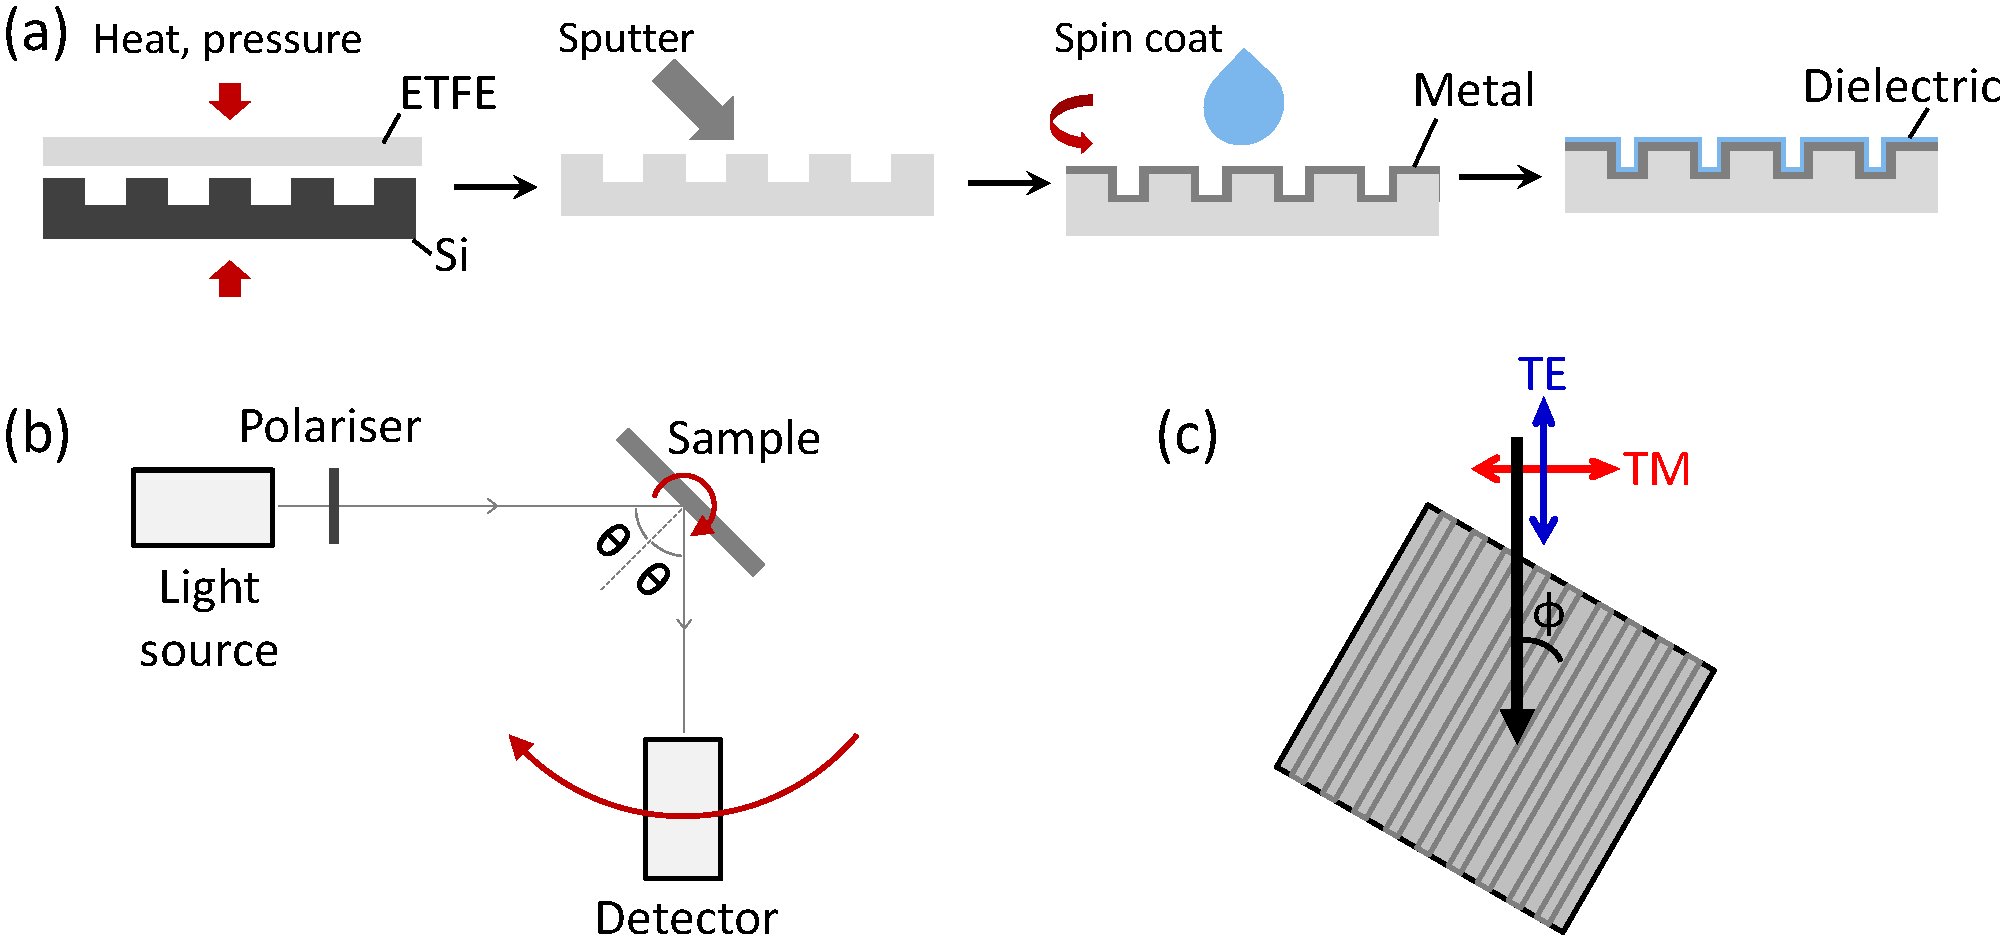
\includegraphics[width=\textwidth]{Fig1}
\caption[(a) Fabrication and (b,c) setup of optical measurements on dielectric-coated metal gratings.]{(a) Fabrication of dielectric-coated metal grating. (b) Setup of angle-dependent reflectivity measurements. (c) Relationship between the polarisation of incoming light (black arrow) and azimuthal angle $\phi$ of the grating orientation. Red/blue arrows indicate the direction of the electric field.}
\label{7Fig1}
\end{figure}
The fabrication of dielectric-coated metal gratings is shown in Fig.\,\ref{7Fig1}(a). Gratings are fabricated in the fluoropolymer ethylene tetrafluoroethylene (ETFE) from nanopatterned silicon stamps using nanoimprinting. A sheet of ETFE (thickness 0.8\,mm) is placed on a silicon stamp with grating periodicity $D$, heated to $200^{\circ}$C and placed under 30\,Bar pressure for 300\,s. The ETFE is cooled to $90^{\circ}$C while maintaining the same pressure, then released from the stamp. An optically opaque metal layer ($\sim$120\,nm thick Ti or Ag) is deposited via sputtering onto the polymer to form metal gratings. Chemically synthesised CHPI powder [Sec.\,\ref{sec:solutiongrowth}] is dissolved in tetrahydrofuran and spin coated onto the gratings in a dehydrated atmosphere to produce a conformal coating. For polystyrene (PS)-coated gratings, $M_w=500000$ PS powder is dissolved in toluene and spin coated onto the gratings. All samples are kept in a nitrogen purge dessication cabinet to prevent oxidation. Measurements by SEM and AFM of the metal and dielectric-coated gratings are used to extract the dimensions of the nanostructures. Polarised specular reflection measurements are made as a function of the incident polar ($\theta$) and azimuthal ($\phi$) angles using a broadband white light source ($215-2500$\,nm) [Figs.\,\ref{7Fig1}(b,c)]. The sample properties are uniform over cm$^2$ areas, with small variations in the depth and morphology of the coatings.

\begin{figure}[h!] 
\centering    
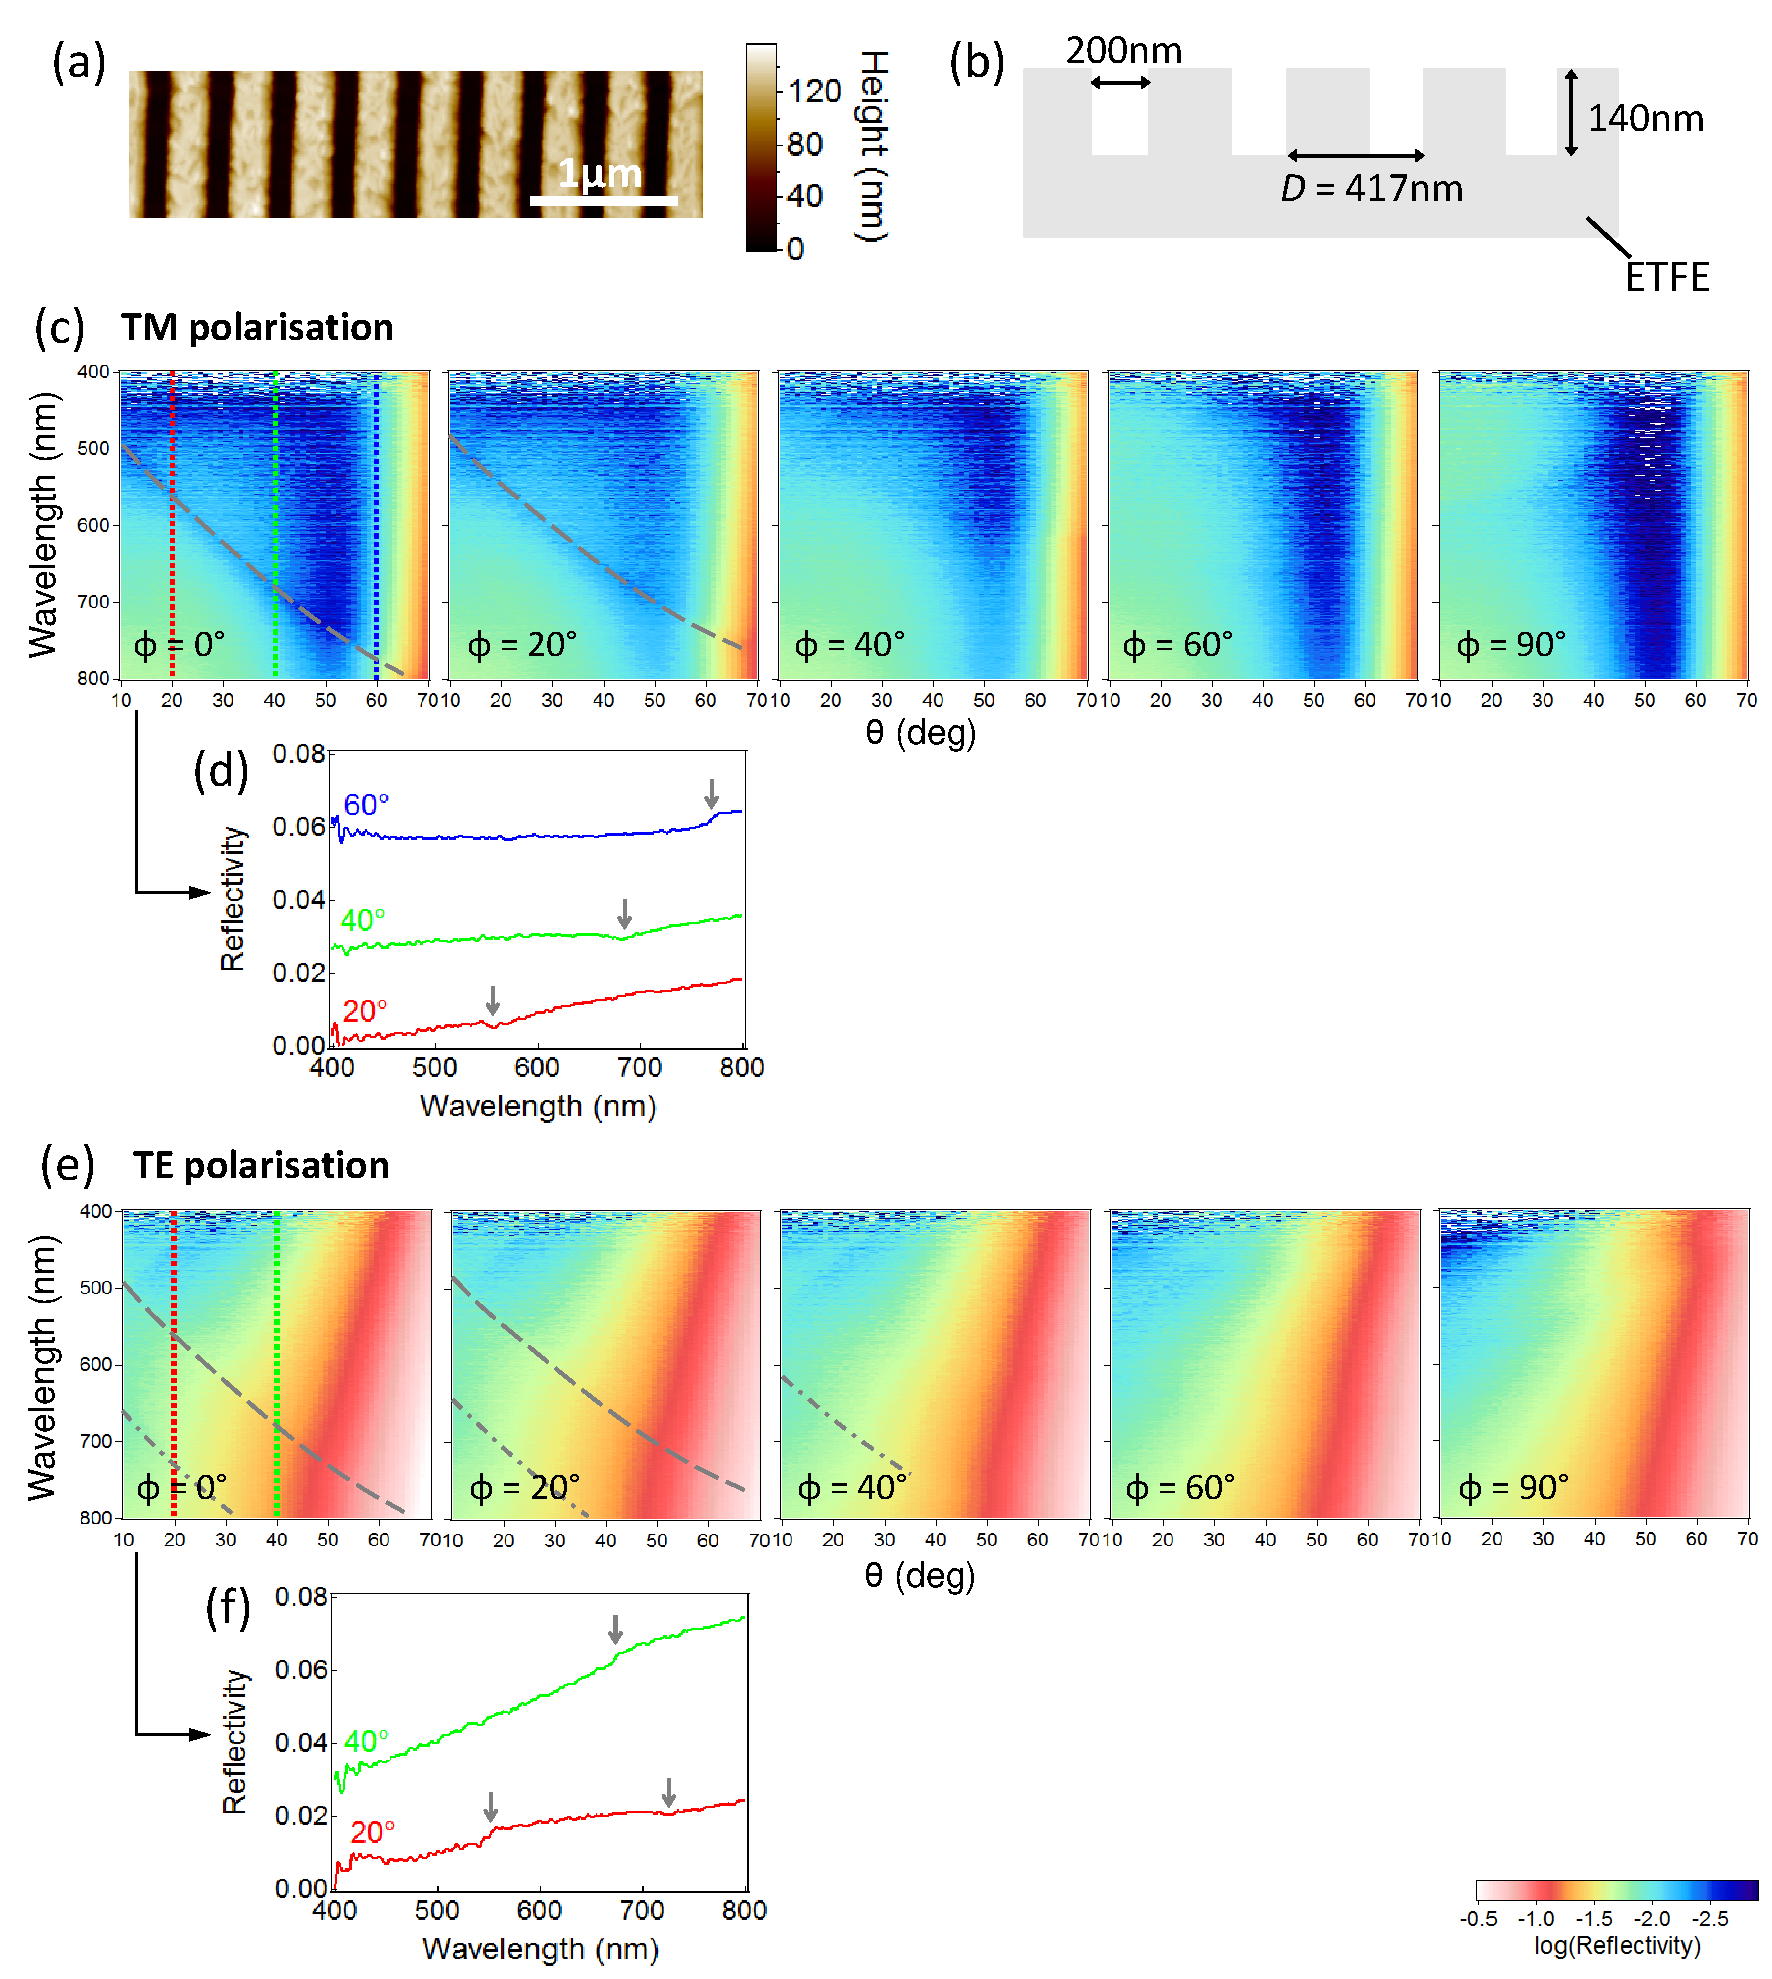
\includegraphics[width=0.95\textwidth]{Fig2}
\caption[(a) AFM image and (b) schematic structure of a $D=417$\,nm ETFE grating. Reflectivity measurements of the ETFE grating in (c,d) TM and (e.f) TE polarisation.]{(a) AFM image and (b) schematic structure of a $D=417$\,nm ETFE grating. (c) TM polarised reflectivity scans of the ETFE grating, and (d) reflectivity spectra for $\phi=0^{\circ}$. Spectra are offset for clarity. (e,f) Same as above for TE polarisation. Photonic grating modes are indicated by grey lines/arrows on reflectivity scans/spectra. For mode assignment see text.}
\label{7Fig2}
\end{figure}
\section{Dielectric gratings}
\subsection{ETFE gratings}
AFM scans of the imprinted $D=417$\,nm ETFE grating [Fig.\,\ref{7Fig2}(a)] show a square-wave grating profile with depth 140\,nm and slit width 200\,nm [Fig.\,\ref{7Fig2}(b)]. TM and TE polarised reflectivity scans show photonic modes of order $m=-1$ in air according to Eq.\,\ref{GratingDisp} [grey dashed lines on Figs.\,\ref{7Fig2}(c,e)] appearing as dips in the reflectivity [Figs.\,\ref{7Fig2}(d,f)]. In TE polarisation we also see the appearance of a redshifted photonic mode [grey dot-dashed line on Fig.\,\ref{7Fig2}(e)], attributed to light that has penetrated the transmissive ETFE. This mode fits well to Eq.\,\ref{GratingDisp} with $n=1.4$, the reported ETFE refractive index \cite{French2011}. For both polarisations the grating modes are no longer visible for $\phi>60^{\circ}$. Note also a dip in the reflectivity of TM scans at $\theta\approx50^{\circ}$ due to the Brewster angle of ETFE.

\subsection{CHPI-coated ETFE gratings}
\begin{figure}[h!p] 
\centering    
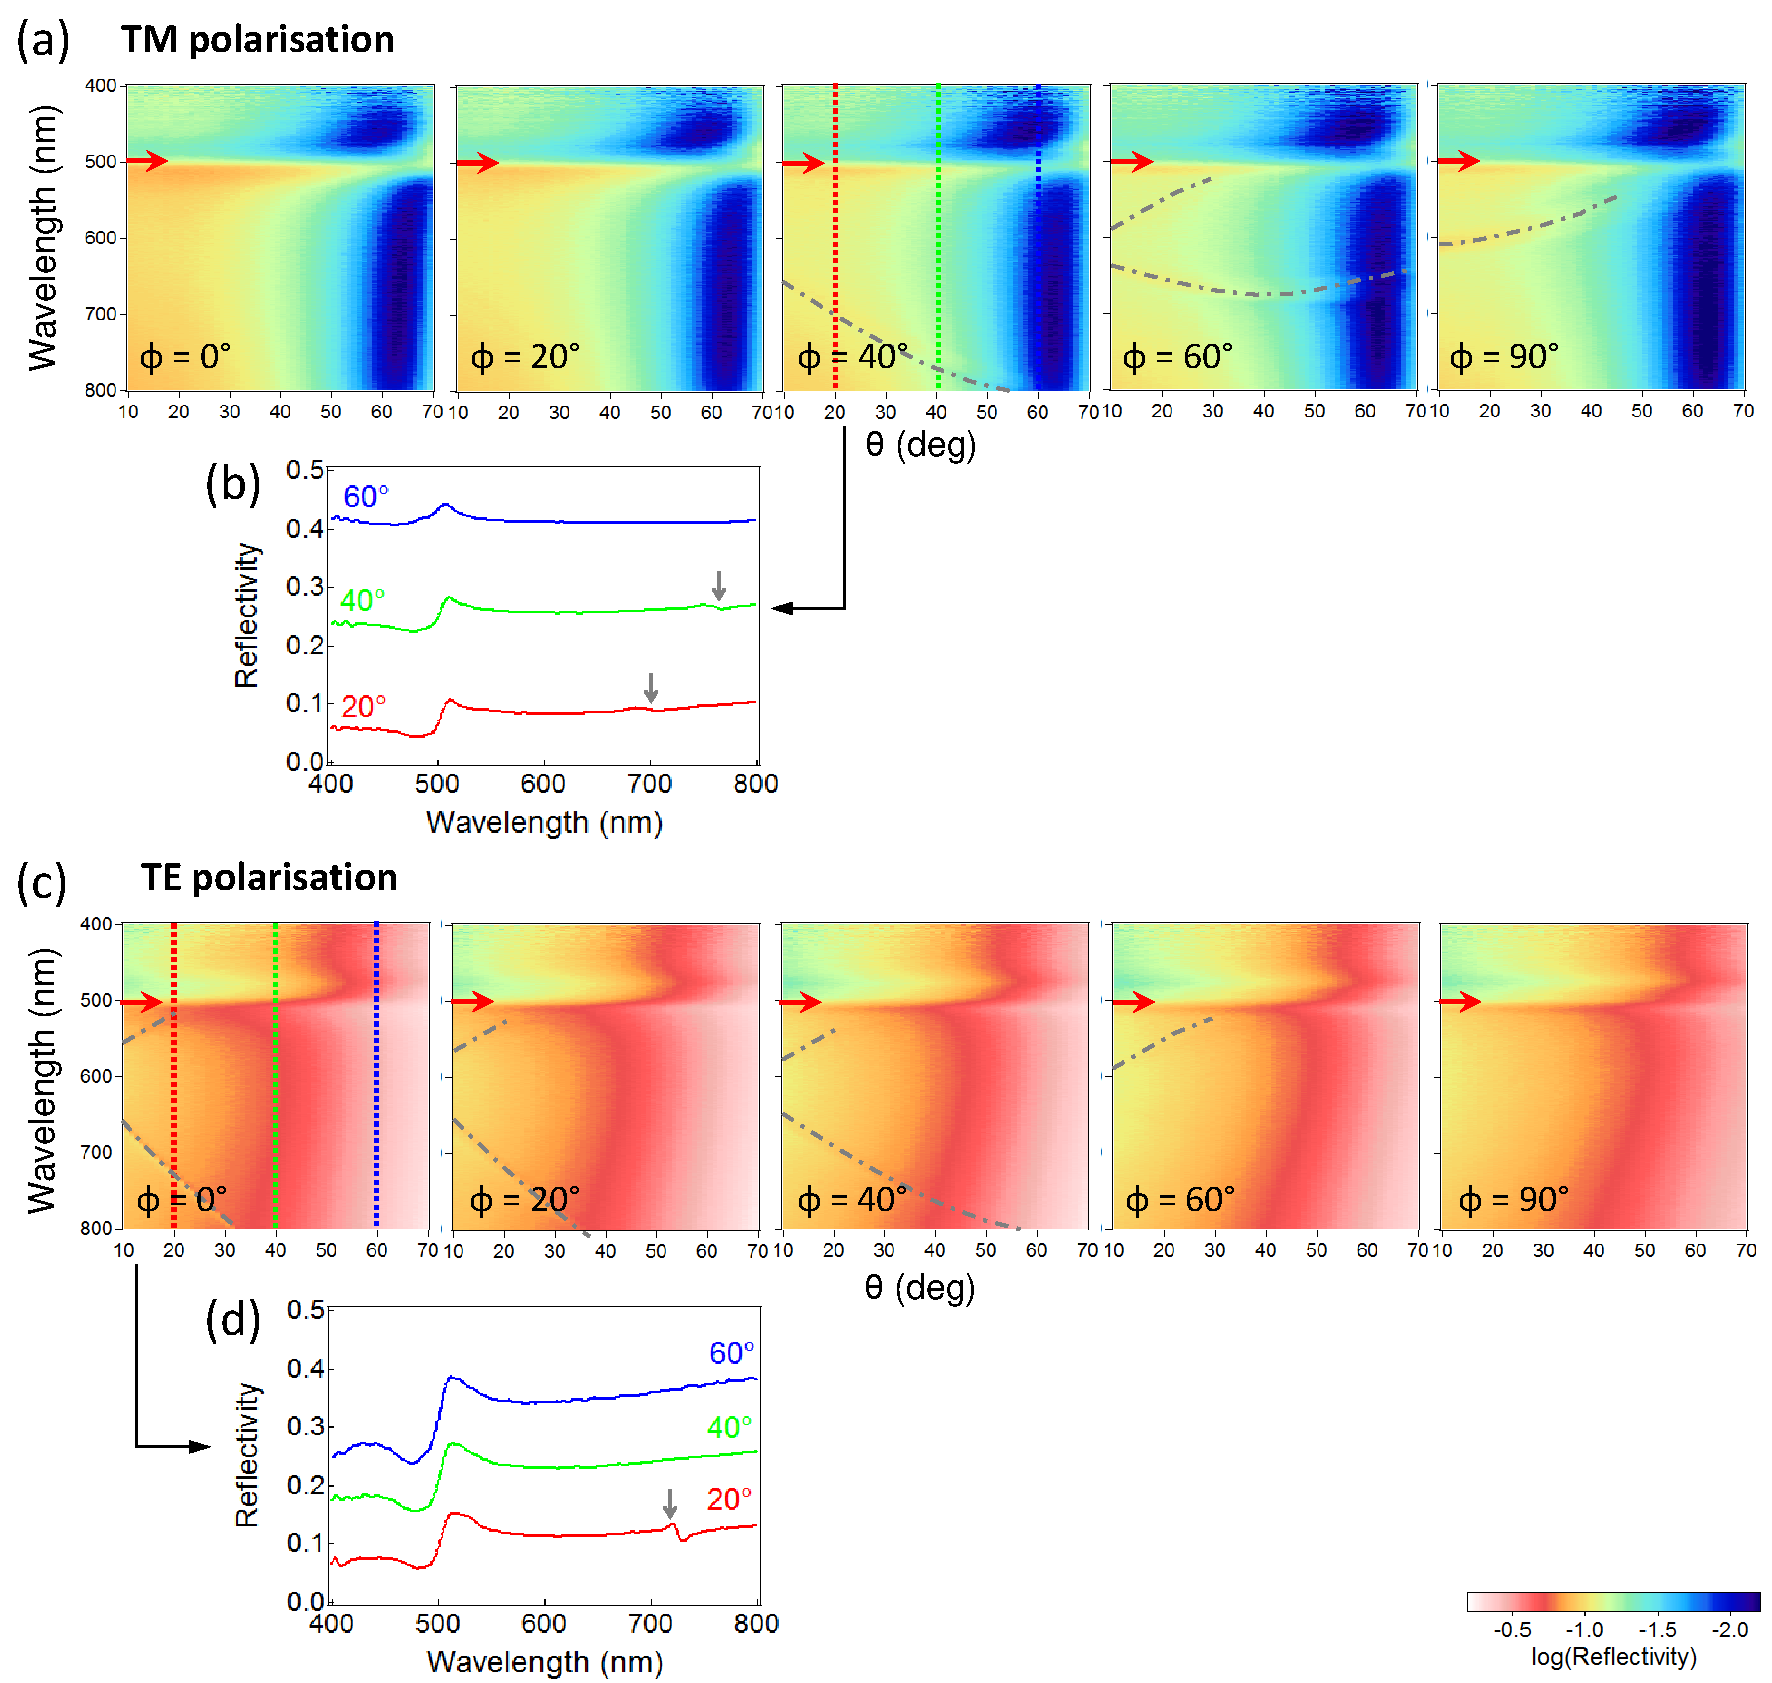
\includegraphics[width=\textwidth]{Fig3}
\caption[Reflectivity measurements of a $D=417$\,nm CHPI-coated ETFE grating in (a,b) TM and (c,d) TE polarisation.]{(a) TM polarised reflectivity scans of a $D=417$\,nm CHPI-coated ETFE grating, and (b) reflectivity spectra for $\phi=40^{\circ}$. Spectra are offset for clarity. (c) Same as (a) for TE polarisation and (d) reflectivity spectra for $\phi=0^{\circ}$. Photonic grating modes are indicated by grey lines/arrows on reflectivity scans/spectra, and excitons by red arrows.}
\label{7Fig3}
\end{figure}
The exciton resonance at 505\,nm dominates both the TM and TE reflectivity scans of CHPI-coated $D=417$\,nm ETFE gratings [Figs.\,\ref{7Fig3}(a,c)]. The $m=\pm1,\,n=1.4$ diffractive photonic grating modes are again visible [grey dot-dashed lines on Figs.\,\ref{7Fig3}(a,c)], and appear as Fano resonances in reflectivity [Figs.\,\ref{7Fig3}(b,d)]. In TM polarisation the diffractive modes are strongest for $\phi=90^{\circ}$, while for TE they are strongest at $\phi=0^{\circ}$, thus coupling with photons is strongest when the $\vec{E}$-field is parallel to grating lines. Note that there are no interactions between grating modes and excitons in this system. The Brewster angle in TM scans has now changed to $\theta\approx62^{\circ}$ due to the larger refractive index of CHPI.


\begin{figure}[h!] 
\centering    
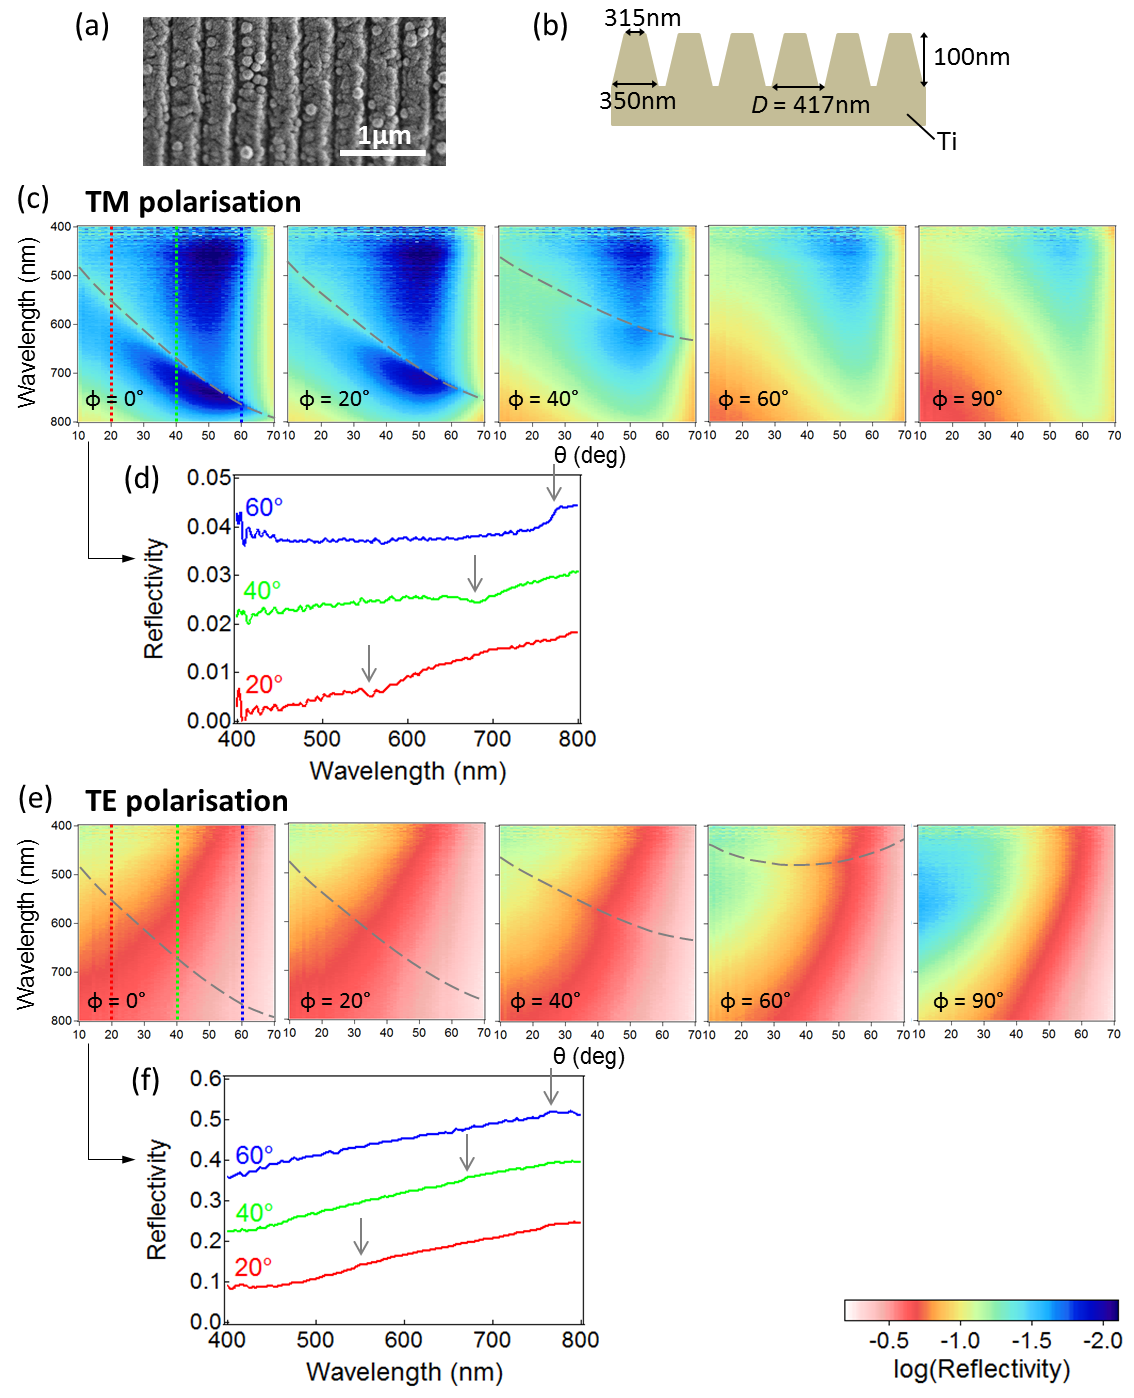
\includegraphics[width=\textwidth]{Fig4}
\caption[(a) SEM image and (b) schematic structure of $D=417$\,nm Ti grating. Reflectivity measurements of Ti grating in (c,d) TM and (e.f) TE polarisation.]{(a) SEM image and (b) schematic structure of a $D=417$\,nm Ti grating. (c) TM polarised reflectivity scans of the Ti grating, and (d) reflectivity spectra for $\phi=0^{\circ}$. Spectra are offset for clarity. (e,f) Same as above for TE polarisation. Photonic grating modes are indicated by grey lines/arrows on reflectivity scans/spectra.}
\label{7Fig4}
\end{figure}
\section{Non-plasmonic metal gratings}
\subsection{Ti gratings}
The SEM image of a $D=417$\,nm Ti grating shows roughness in the sputtered Ti film on ETFE [Fig.\,\ref{7Fig4}(a)], while AFM measurements reveal a trapezoidal grating profile as a result of the nanoimprinting process. Heating and cooling of ETFE during sputtering also appears to have changed the grating periodicity $D$, as the photonic grating modes in reflectivity scans [Figs.\,\ref{7Fig4}(c,e)] are best fit to $D=410$\,nm [Eq.\,\ref{GratingDisp}]. Aside from the change in geometry, the appearance of $m=-1$ grating modes in optical spectra is very similar to what was observed in ETFE gratings, with modes appearing as dips in reflectivity. However the coupling to photons is much weaker in TE polarisation, particularly at $\phi=0^{\circ}$ as the $\vec{E}$-field is parallel to grating lines [Sec.\,\ref{sec:plasmonicgratings}].



\subsection{CHPI-coated Ti gratings}
Polarised reflectivity spectra of a CHPI-coated planar Ti film [Fig.\,\ref{7Fig5}] show the appearance of an exciton resonance at 505\,nm, indicating the excitons are unaffected by the metal film below. The experimental data fits well to transfer matrix simulations \cite{Born1999} of 70\,nm CHPI-coated 120\,nm Ti film, and the differences observed can be attributed to non-uniformity and roughness in both the CHPI and Ti films.
\begin{figure}[h!] 
\centering    
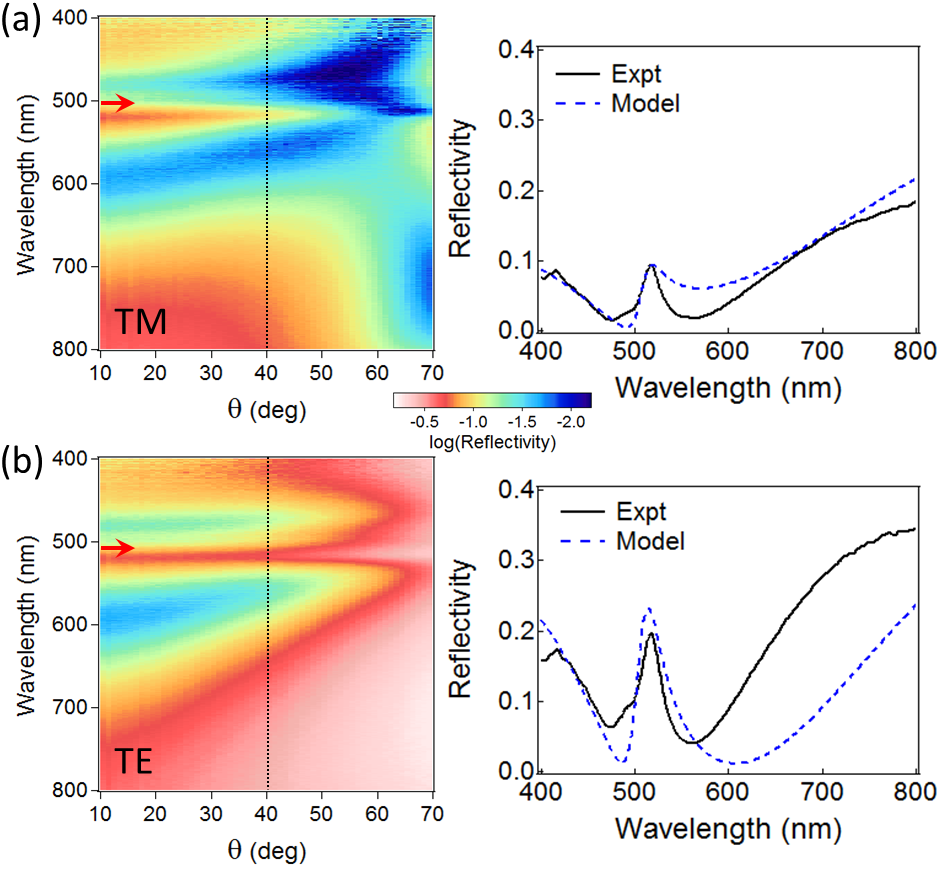
\includegraphics[width=0.72\textwidth]{Fig5}
\caption[(a) TM and (b) TE polarised reflectivity scans of 70\,nm CHPI film on 120\,nm planar Ti film compared to transfer matrix simulations.]{Specular reflectivity scans of a 70\,nm CHPI-coated 120\,nm planar Ti film (left) with (a) TM and (b) TE polarised light. Excitons are marked by red arrows. Spectra at $\theta=40^{\circ}$ are plotted with those predicted by transfer matrix simulations (right).}
\label{7Fig5}
\end{figure}

\begin{figure}[h!] 
\centering    
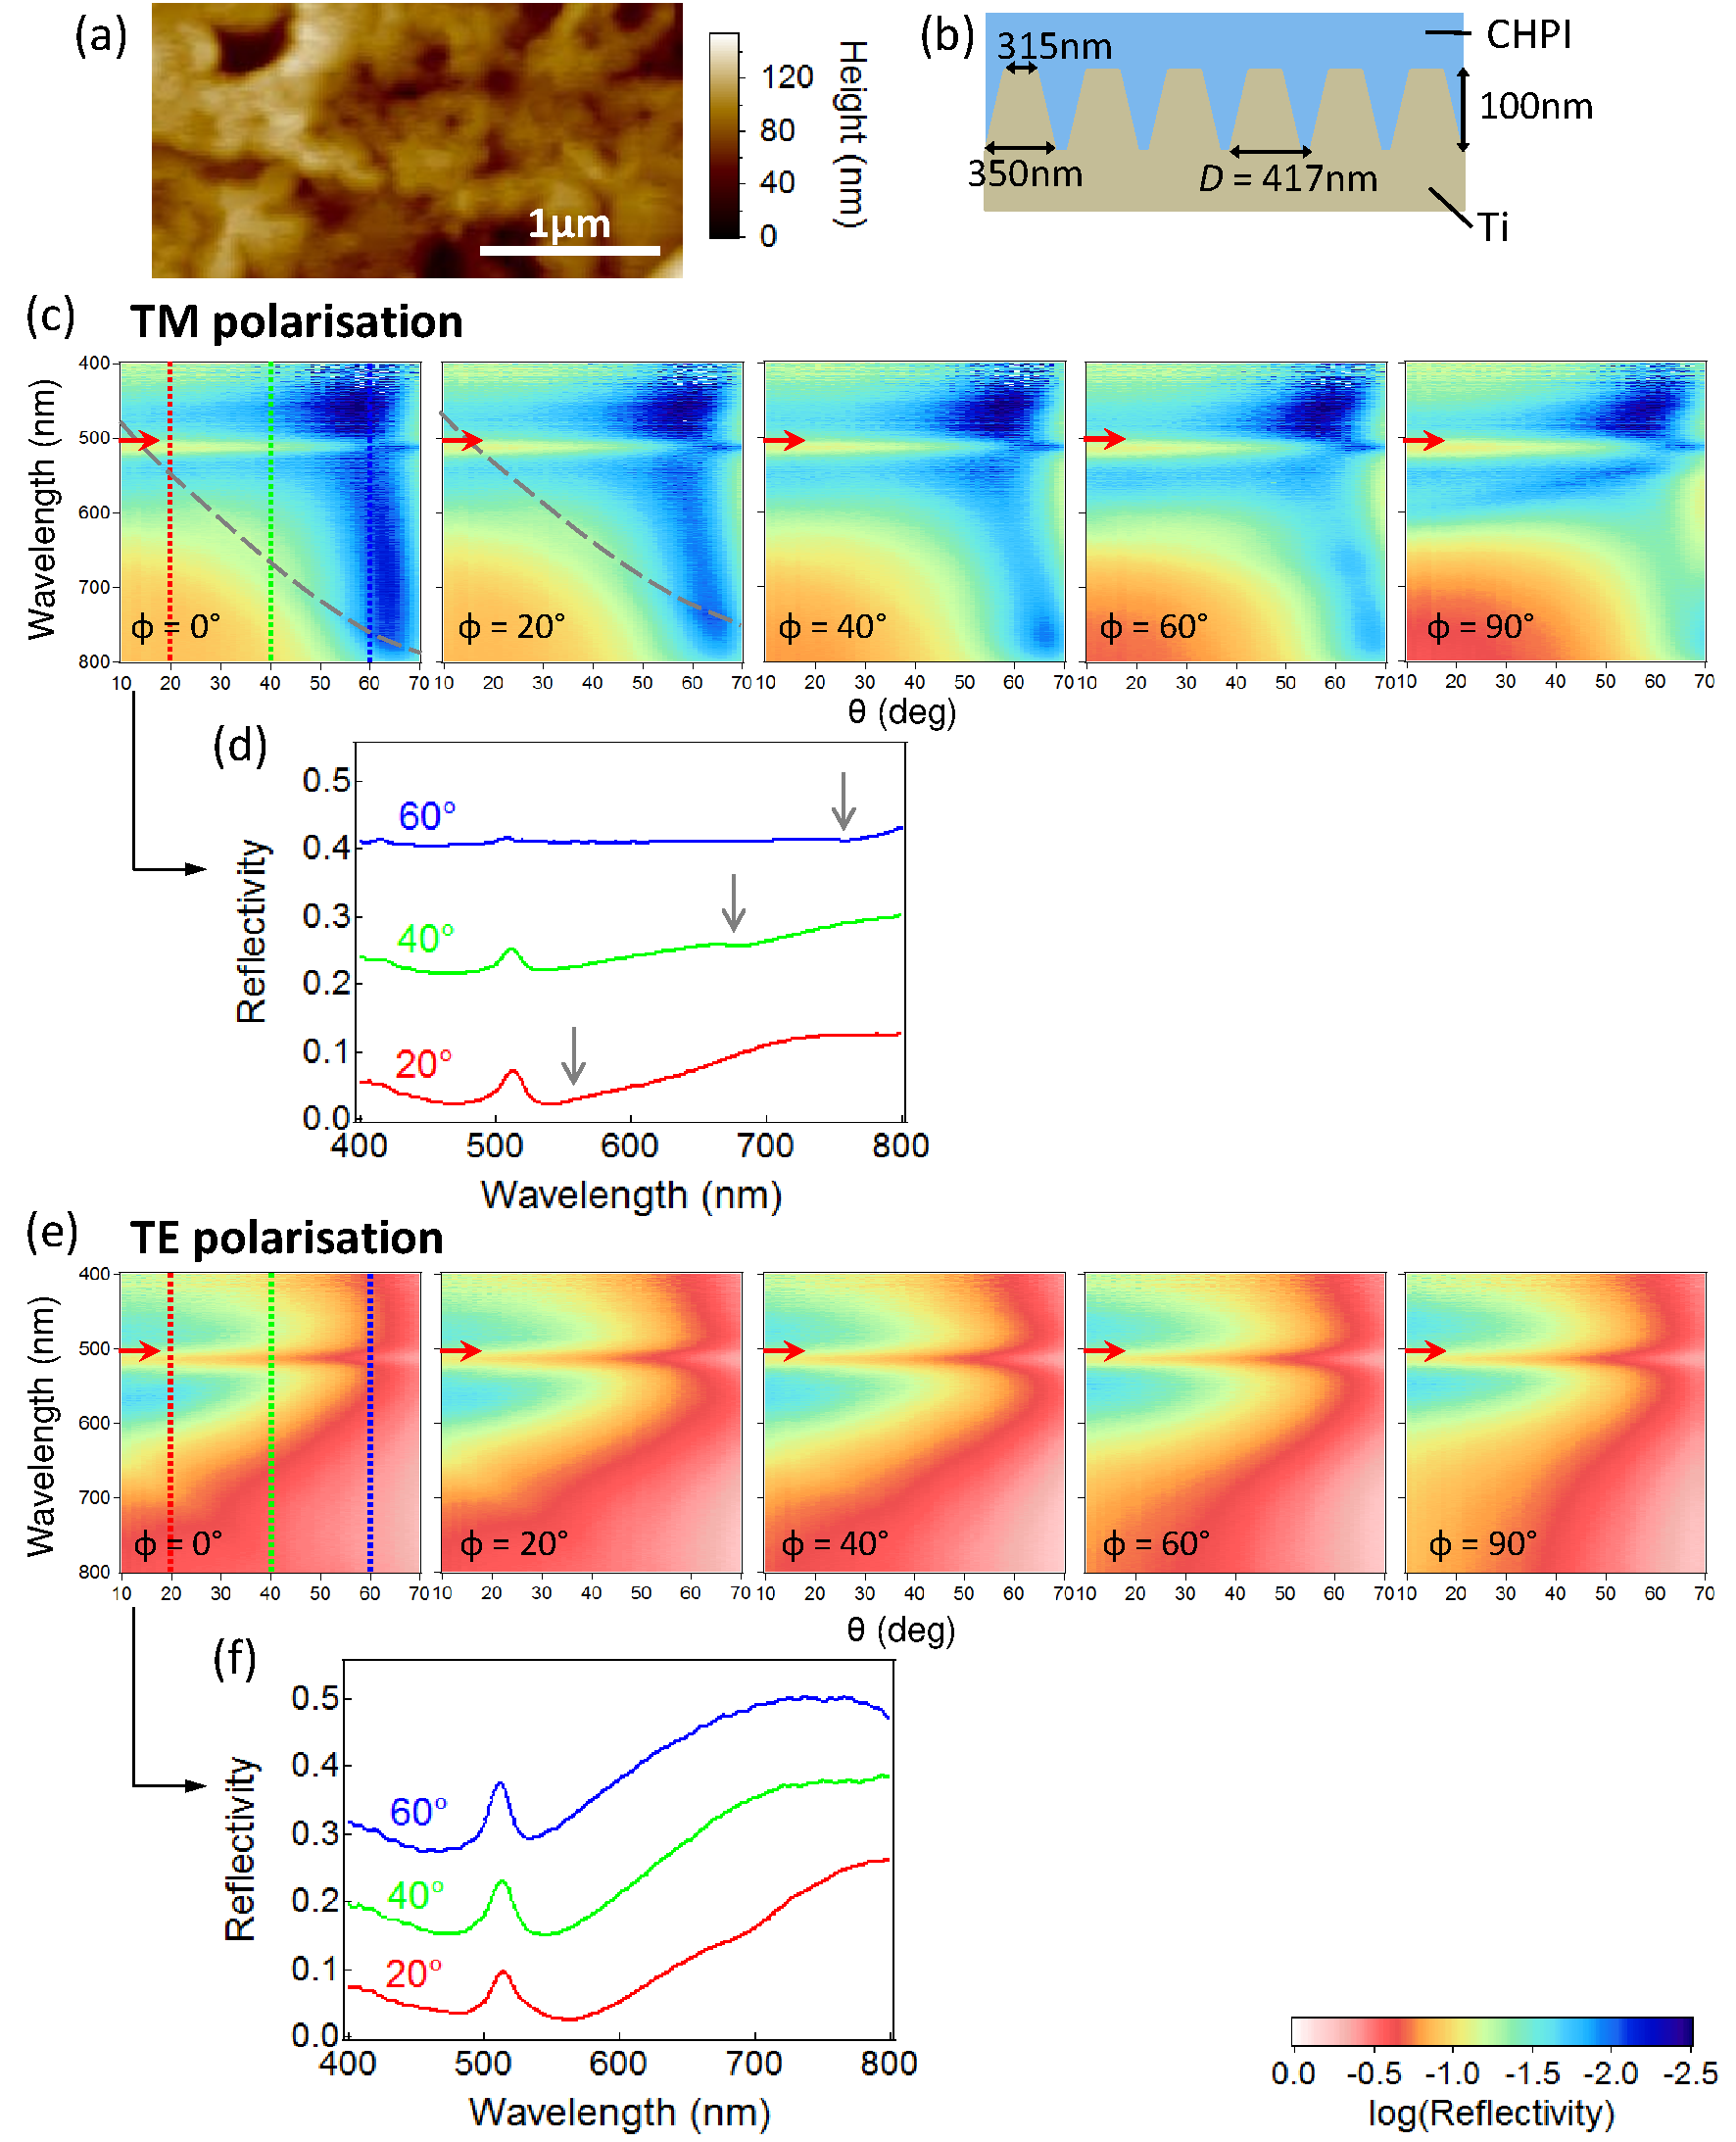
\includegraphics[width=0.95\textwidth]{Fig6}
\caption[(a) AFM image and (b) schematic structure of $D=417$\,nm CHPI-coated Ti grating. Reflectivity measurements of CHPI-coated Ti grating in (c,d) TM and (e.f) TE polarisation.]{(a) AFM image and (b) schematic structure of a $D=417$\,nm CHPI-coated Ti grating. (c) TM polarised reflectivity scans of the CHPI-coated Ti grating, and (d) reflectivity spectra for $\phi=0^{\circ}$. Spectra are offset for clarity. (e,f) Same as above for TE polarisation. Photonic grating modes are indicated by grey lines/arrows on reflectivity scans/spectra, and excitons by red arrows.}
\label{7Fig6}
\end{figure}
AFM measurements show that the metal grating is completely immersed in a non-uniform coating for the $D=417$\,nm CHPI-coated Ti grating [Figs.\,\ref{7Fig6}(a,b)]. As with CHPI-coated ETFE gratings, the exciton resonance at 505\,nm dominates reflectivity spectra for both polarisations [Figs.\,\ref{7Fig6}(c,e)]. Although very weak dips can be seen to indicate diffractive $m=-1$ grating modes in TM polarisation [Fig.\,\ref{7Fig6}(d)], coupling of TE-polarised light to grating modes is so weak that spectra appear almost identical to that of a CHPI-coated planar Ti film [Figs.\,\ref{7Fig5}(b) and \ref{7Fig6}(f)]. In both cases there are no interactions between CHPI excitons and modes of the non-plasmonic Ti grating.

\begin{figure}[h!] 
\centering    
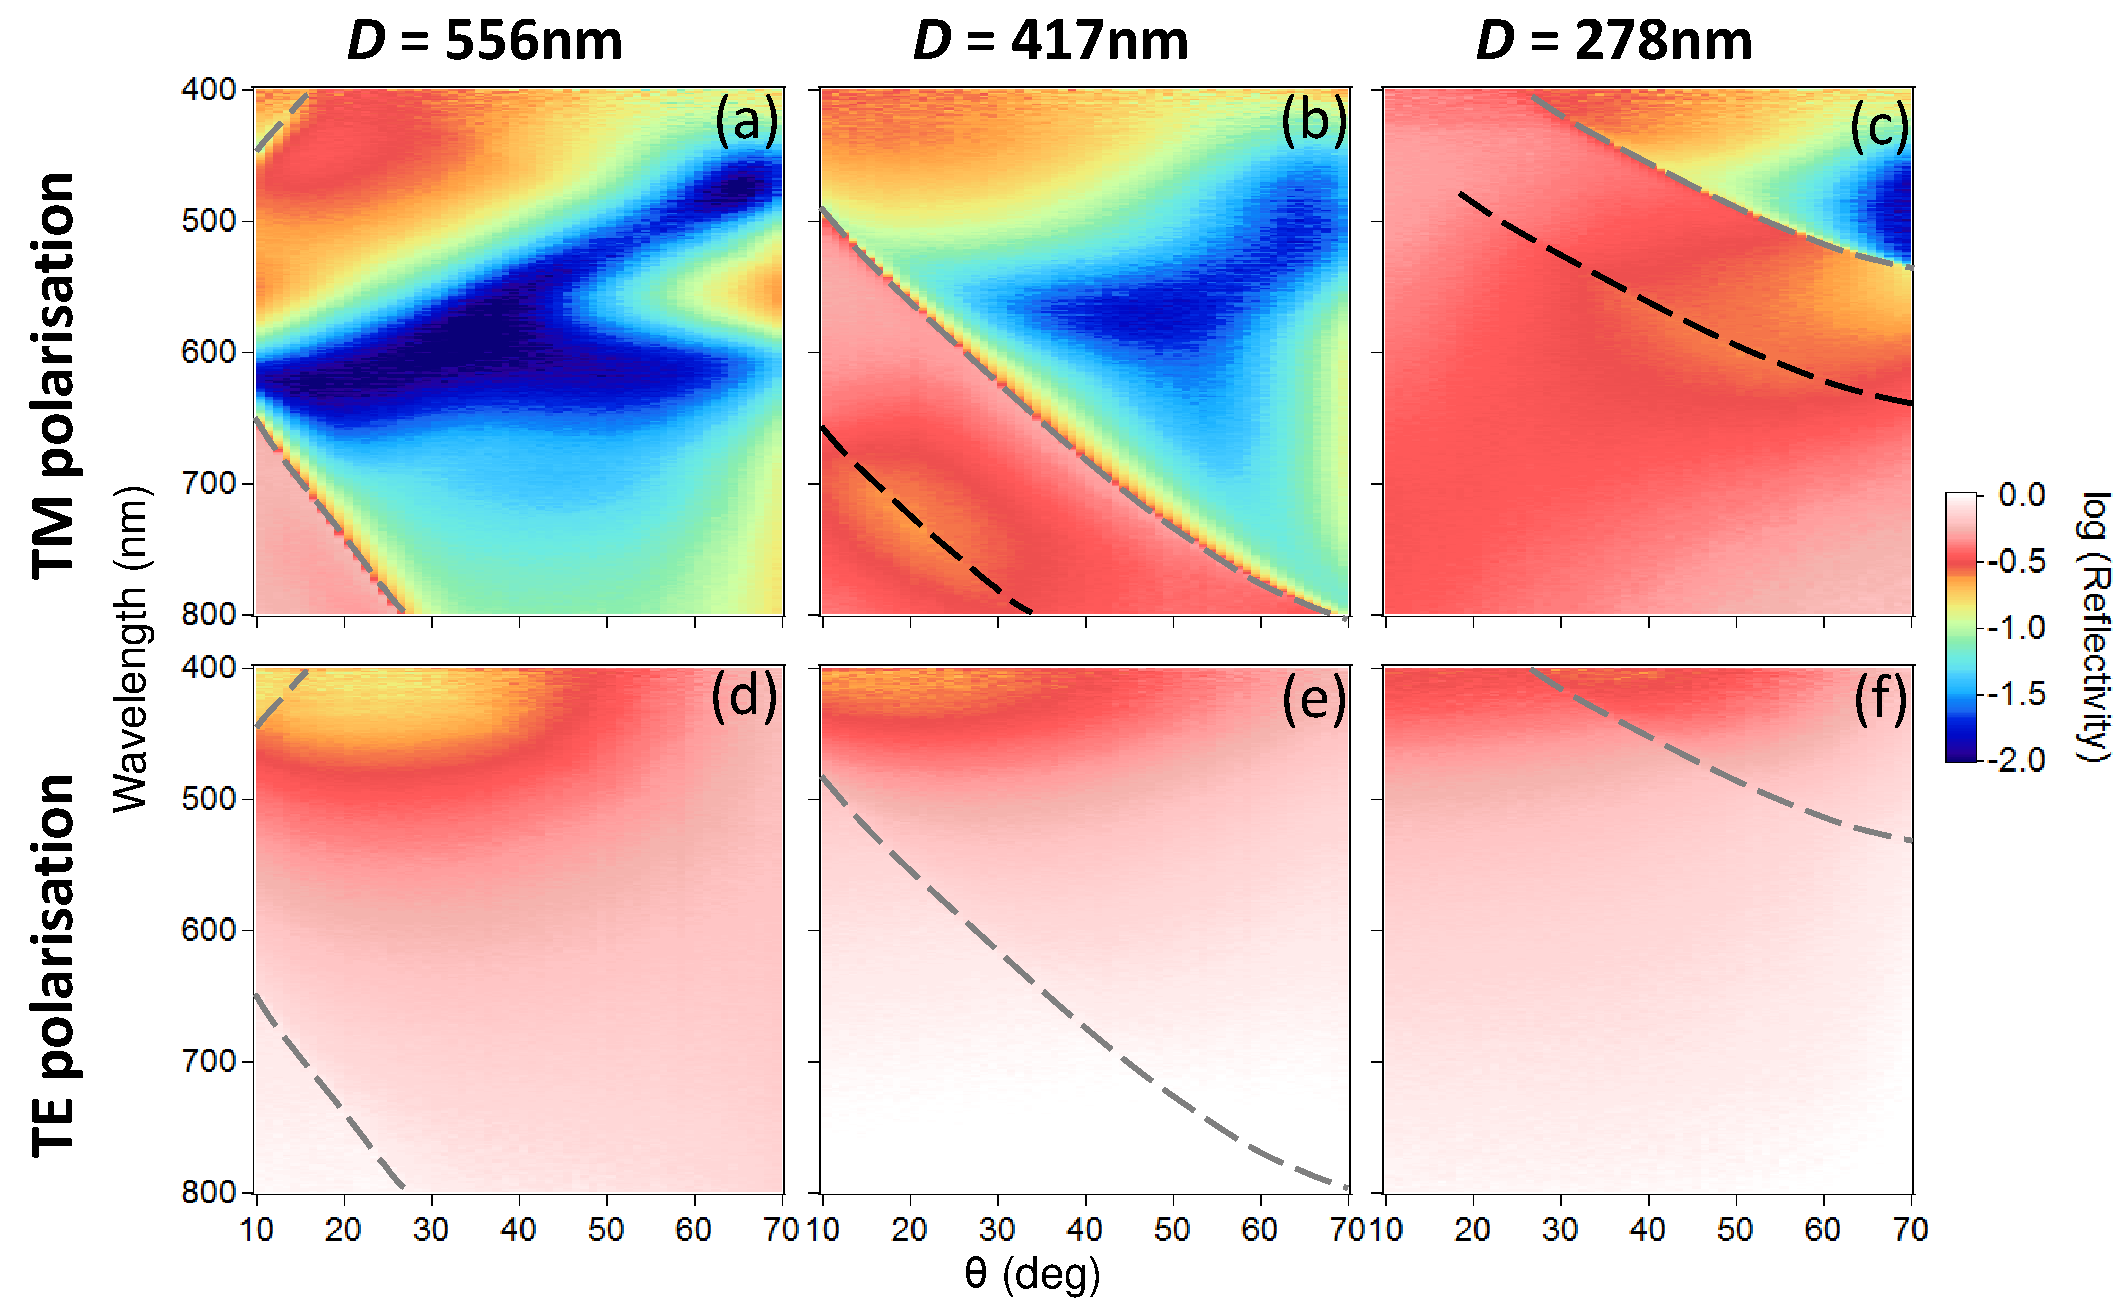
\includegraphics[width=\textwidth]{Fig7}
\caption[TM and TE specular reflectivity scans of uncoated Ag gratings at $\phi=0^{\circ}$, $D=556$, 417 and 278\,nm.]{Specular reflectivity scans of uncoated Ag gratings at $\phi=0^{\circ}$ with periodicity $D$ and polarisation of light as labelled. Photonic grating modes (threshold anomalies) are marked by grey dashed lines, and plasmonic grating modes (resonance anomalies) are marked by black dashed lines.}
\label{7Fig7}
\end{figure}
\section{Plasmonic metal gratings}

\subsection{Ag gratings}
Fig.\,\ref{7Fig7} shows reflectivity scans at $\phi=0^{\circ}$ for Ag gratings, $D=556$, 417 and 278\,nm. The spectra for all three gratings show the same features: in TM polarisation a sharp threshold anomaly whose dispersion follows Eq.\,\ref{GratingDisp} for $m=\pm1$ (grey dashed lines) and a redshifted dip for the resonance anomaly indicating the presence of excited SPPs (black dashed lines). In TE polarisation we don't observe any anomaly features due to the inability to excite SPPs, instead we see the $m=\pm1$ photonic modes [Sec.\,\ref{sec:plasmonicgratings}].


\begin{figure}[h!] 
\centering    
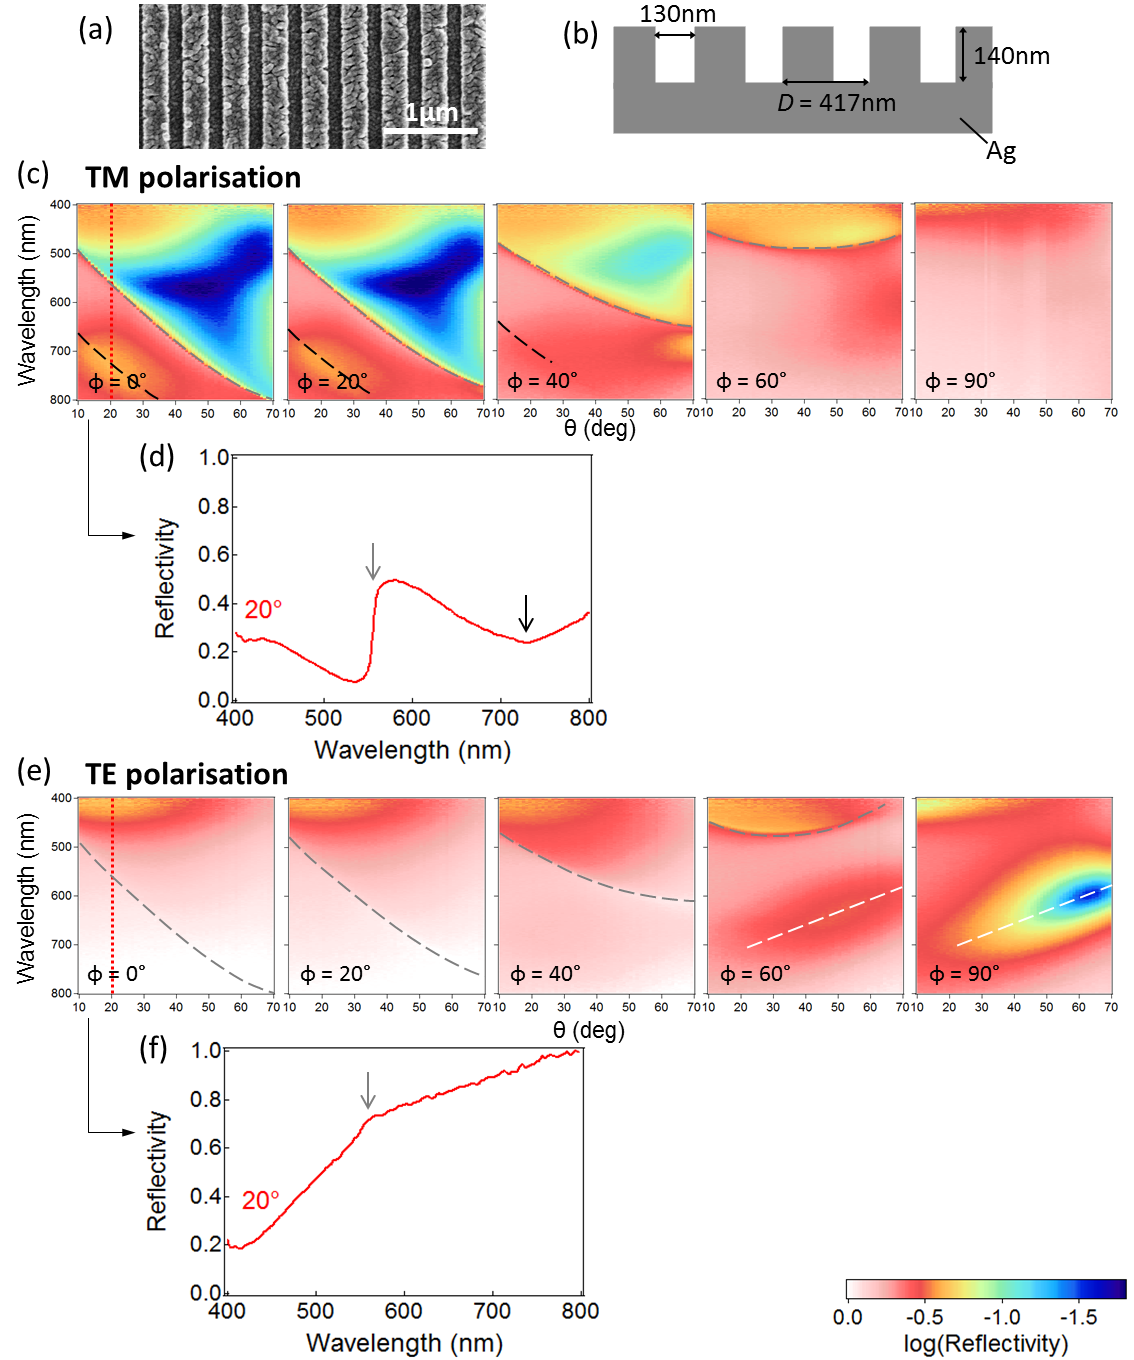
\includegraphics[width=0.95\textwidth]{Fig8}
\caption[(a) SEM image and (b) schematic structure of $D=417$\,nm Ag grating. Reflectivity measurements of Ag grating in (c,d) TM and (e.f) TE polarisation.]{(a) SEM image and (b) schematic structure of a $D=417$\,nm Ag grating. (c) TM polarised reflectivity scans of the Ag grating, and (d) reflectivity spectra for $\phi=0^{\circ}$. (e,f) Same as above for TE polarisation. Photonic grating modes (threshold anomalies) are indicated by grey lines/arrows on reflectivity scans/spectra, plasmonic grating modes (resonance anomalies) by black lines/arrows, and Fabry-Perot modes by white dashed lines.}
\label{7Fig8}
\end{figure}

\begin{figure}[h!p] 
\centering    
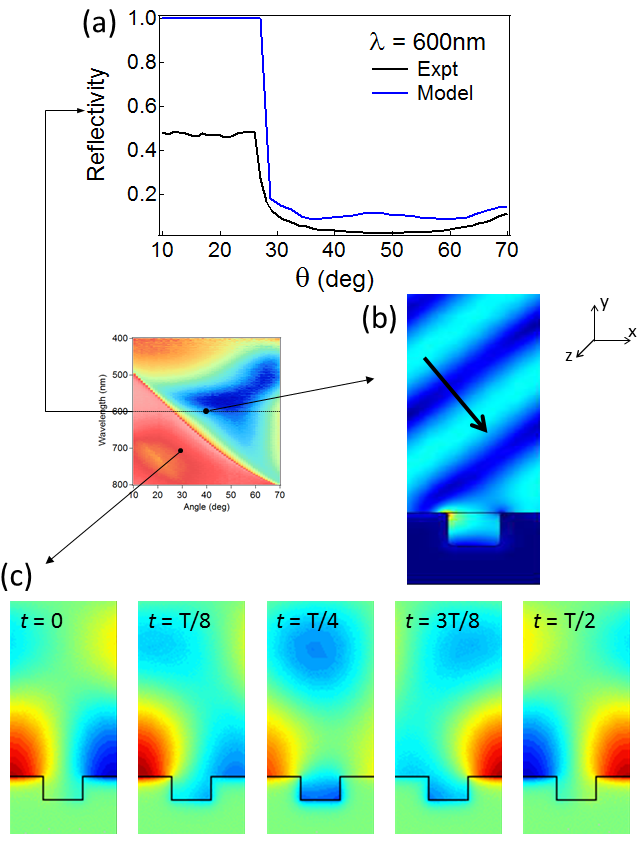
\includegraphics[width=0.8\textwidth]{Fig9}
\caption{(a) Experimental and modelled TM reflectivity spectra of the $D=417$\,nm Ag grating for $\phi=0^{\circ}$,\,$\lambda=600$\,nm. (b) $\vec{E}$-field intensity ($\vec{E}\cdot\vec{E}$) profile for $\lambda=600$\,nm$,\,$\theta=40^{\circ}$. The direction of the incident light is shown by the black arrow. (c) $H_z$ nearfield profile at time $t$ of the optical cycle T for $\lambda=700$\,nm$,\,	\theta=30^{\circ}$.}
\label{7Fig9}
\end{figure}
Focusing on the $D=417$\,nm grating, we see that the sputtered Ag film on ETFE shows some roughness [Fig.\,\ref{7Fig8}(a)], and AFM measurements indicate a square-wave grating with depth 140\,nm and slit width 130\,nm [Fig.\,\ref{7Fig8}(b)]. In reflectivity the threshold anomalies (grey dashed lines) shift as expected according to Eq.\,\ref{GratingDisp} in TM polarisation [Fig.\,\ref{7Fig8}(c)], and appear as sharp changes in the intensity [Fig.\,\ref{7Fig8}(d)]. The redshifted resonance anomalies (black dashed lines) become weaker with increasing $\phi$ and are no longer observed when $\phi>60^{\circ}$ as the $\vec{E}$-field polarisation makes it harder for photons to couple to SPPs. For the same reason no anomalies are observed in TE polarisation at low $\phi$, where the photonic modes appear weakly in spectra [Fig.\,\ref{7Fig8}(f)]. We would expect to observe anomalies at $\phi=90^{\circ}$ in TE polarisation, however the energy of the mode is too high for our measurement range here. The broad dips seen at $\phi=60^{\circ}$ and $90^{\circ}$ in TE polarisation (white dashed lines) are assigned to the Fabry-Perot interference mode of light reflected from the top and bottom surfaces of the grating. This mode doesn't change in position with $\phi$ and extrapolates to $\sim700$\,nm at $\theta=0^{\circ}$, which fits the height of the gratings as seen in AFM measurements ($\sim150$\,nm).


In collaboration with Dr.\,David Leipold and Prof.\,Erich Runge from Technische Universit\"{a}t Ilmenau, we use the finite element method (FEM) to model the electromagnetic nearfield of grating modes in order to understand their behaviour. The modelled spectrum for $\phi=0^{\circ}$,\,$\lambda=600$\,nm agrees very well with features of the experimental data [Fig.\,\ref{7Fig9}(a)], but has a larger reflectivity overall as the model does not take into account the Ag film roughness. Low efficiency of the specularly reflected grating order gives rise to the low reflection region seen at high $\theta$, instead the coupling is strongest to the $-1$ diffracted order, and the $\vec{E}$-field intensity in Fig.\,\ref{7Fig9}(b) is produced from the interference between the incident and diffracted light. The modelled $H_z$ field component of the resonance anomaly shows that it does indeed behave like an SPP travelling on the surface of the metal [Fig.\,\ref{7Fig9}(c)].

The position of the threshold anomaly is fixed by the periodicity of the structure, however as the resonance anomaly is caused by the interference between diffracted light and SPPs we expect its position to be much more sensitive to the geometry of the grating. Fig.\,\ref{7Fig10} shows the profiles and TM reflectivity scans at $\phi=0^{\circ}$ of three different gratings, ranging from square-wave [Fig.\,\ref{7Fig10}(a)] to approximately sinusiodal [Figs.\,\ref{7Fig10}(b,c)]. The sharp threshold anomalies (grey dashed lines) remain in the same position for all three gratings, barring small changes in $D$ as a result of the sputtering process. However the widths and positions of the resonance anomalies vary greatly with geometry, and the sharpest resonances are produced by sinusoidal gratings. We also observe a dispersionless mode at $\sim450$\,nm in Figs.\,\ref{7Fig10}(b,c) that may be due to the presence of channel plasmons, which require a narrowing of the grating slit as seen in the sinusoidal gratings [Sec.\,\ref{sec:channel}].
\begin{figure}[h!p] 
\centering    
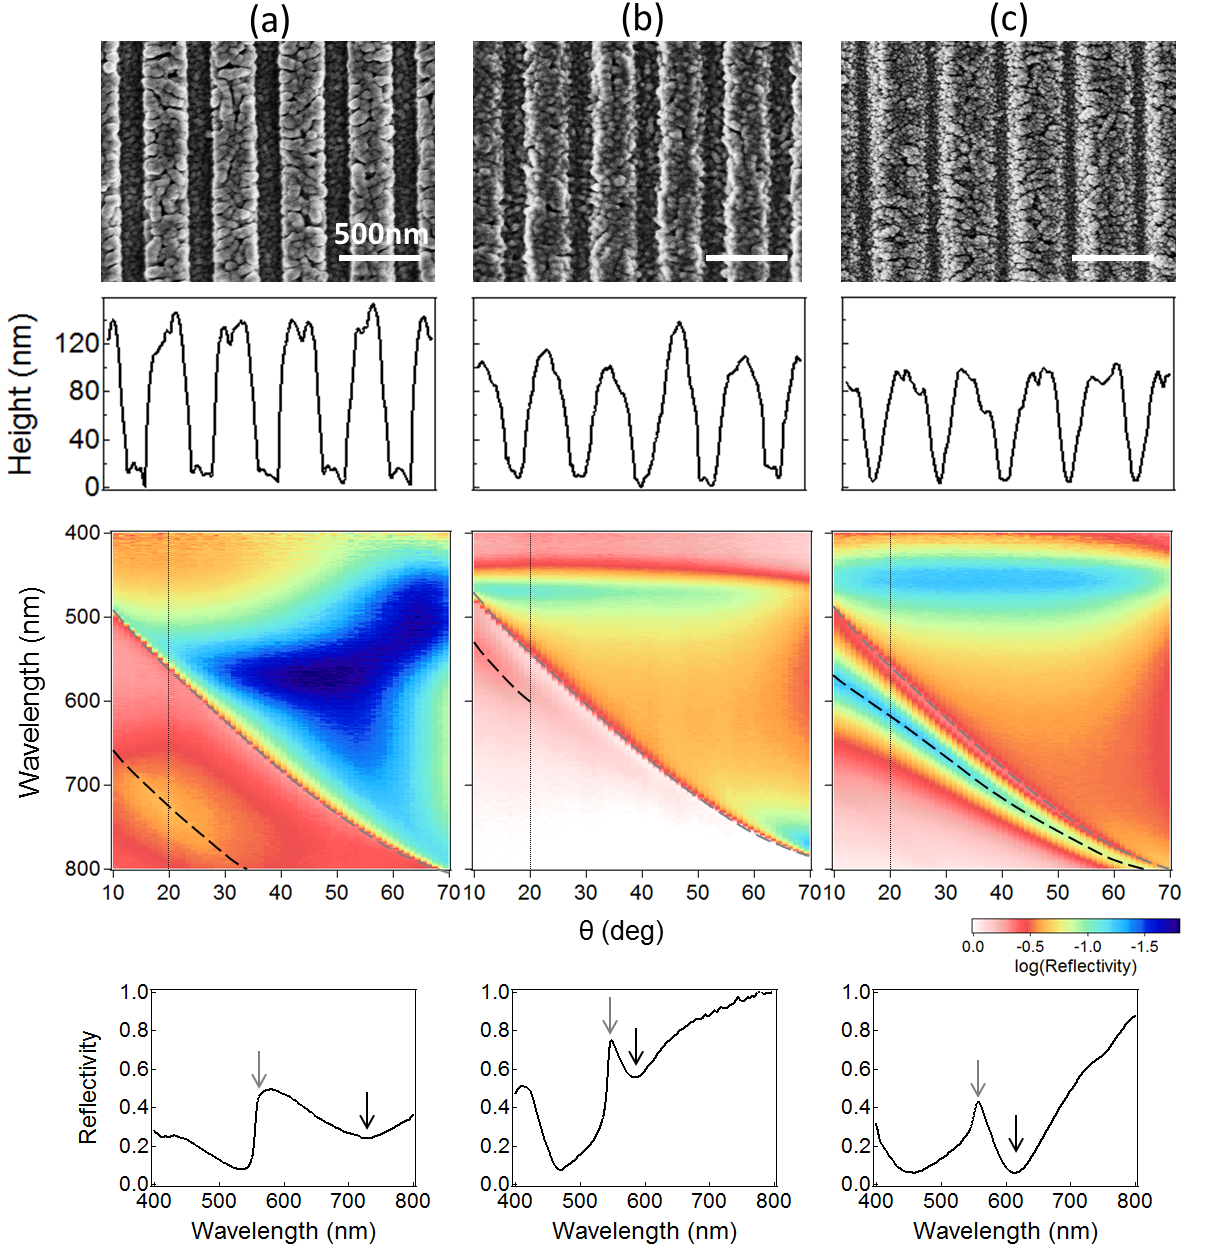
\includegraphics[width=\textwidth]{Fig10}
\caption[Effect of grating geometry on the optical spectra of $D=417$\,nm Ag gratings.] {(From top) SEM image, AFM profile, TM specular reflectivity scans at $\phi=0^{\circ}$, and reflectivity spectra at $\phi=0^{\circ}$ $\theta=20^{\circ}$ for three $D=417$\,nm Ag gratings with increasing sinusoidal profiles (a$\rightarrow$c). Photonic grating modes (threshold anomalies) are marked by grey dashed lines/arrows, and plasmonic grating modes (resonance anomalies) by black dashed lines/arrows on reflectivity scans/spectra.}
\label{7Fig10}
\end{figure}

\begin{figure}[h!] 
\centering    
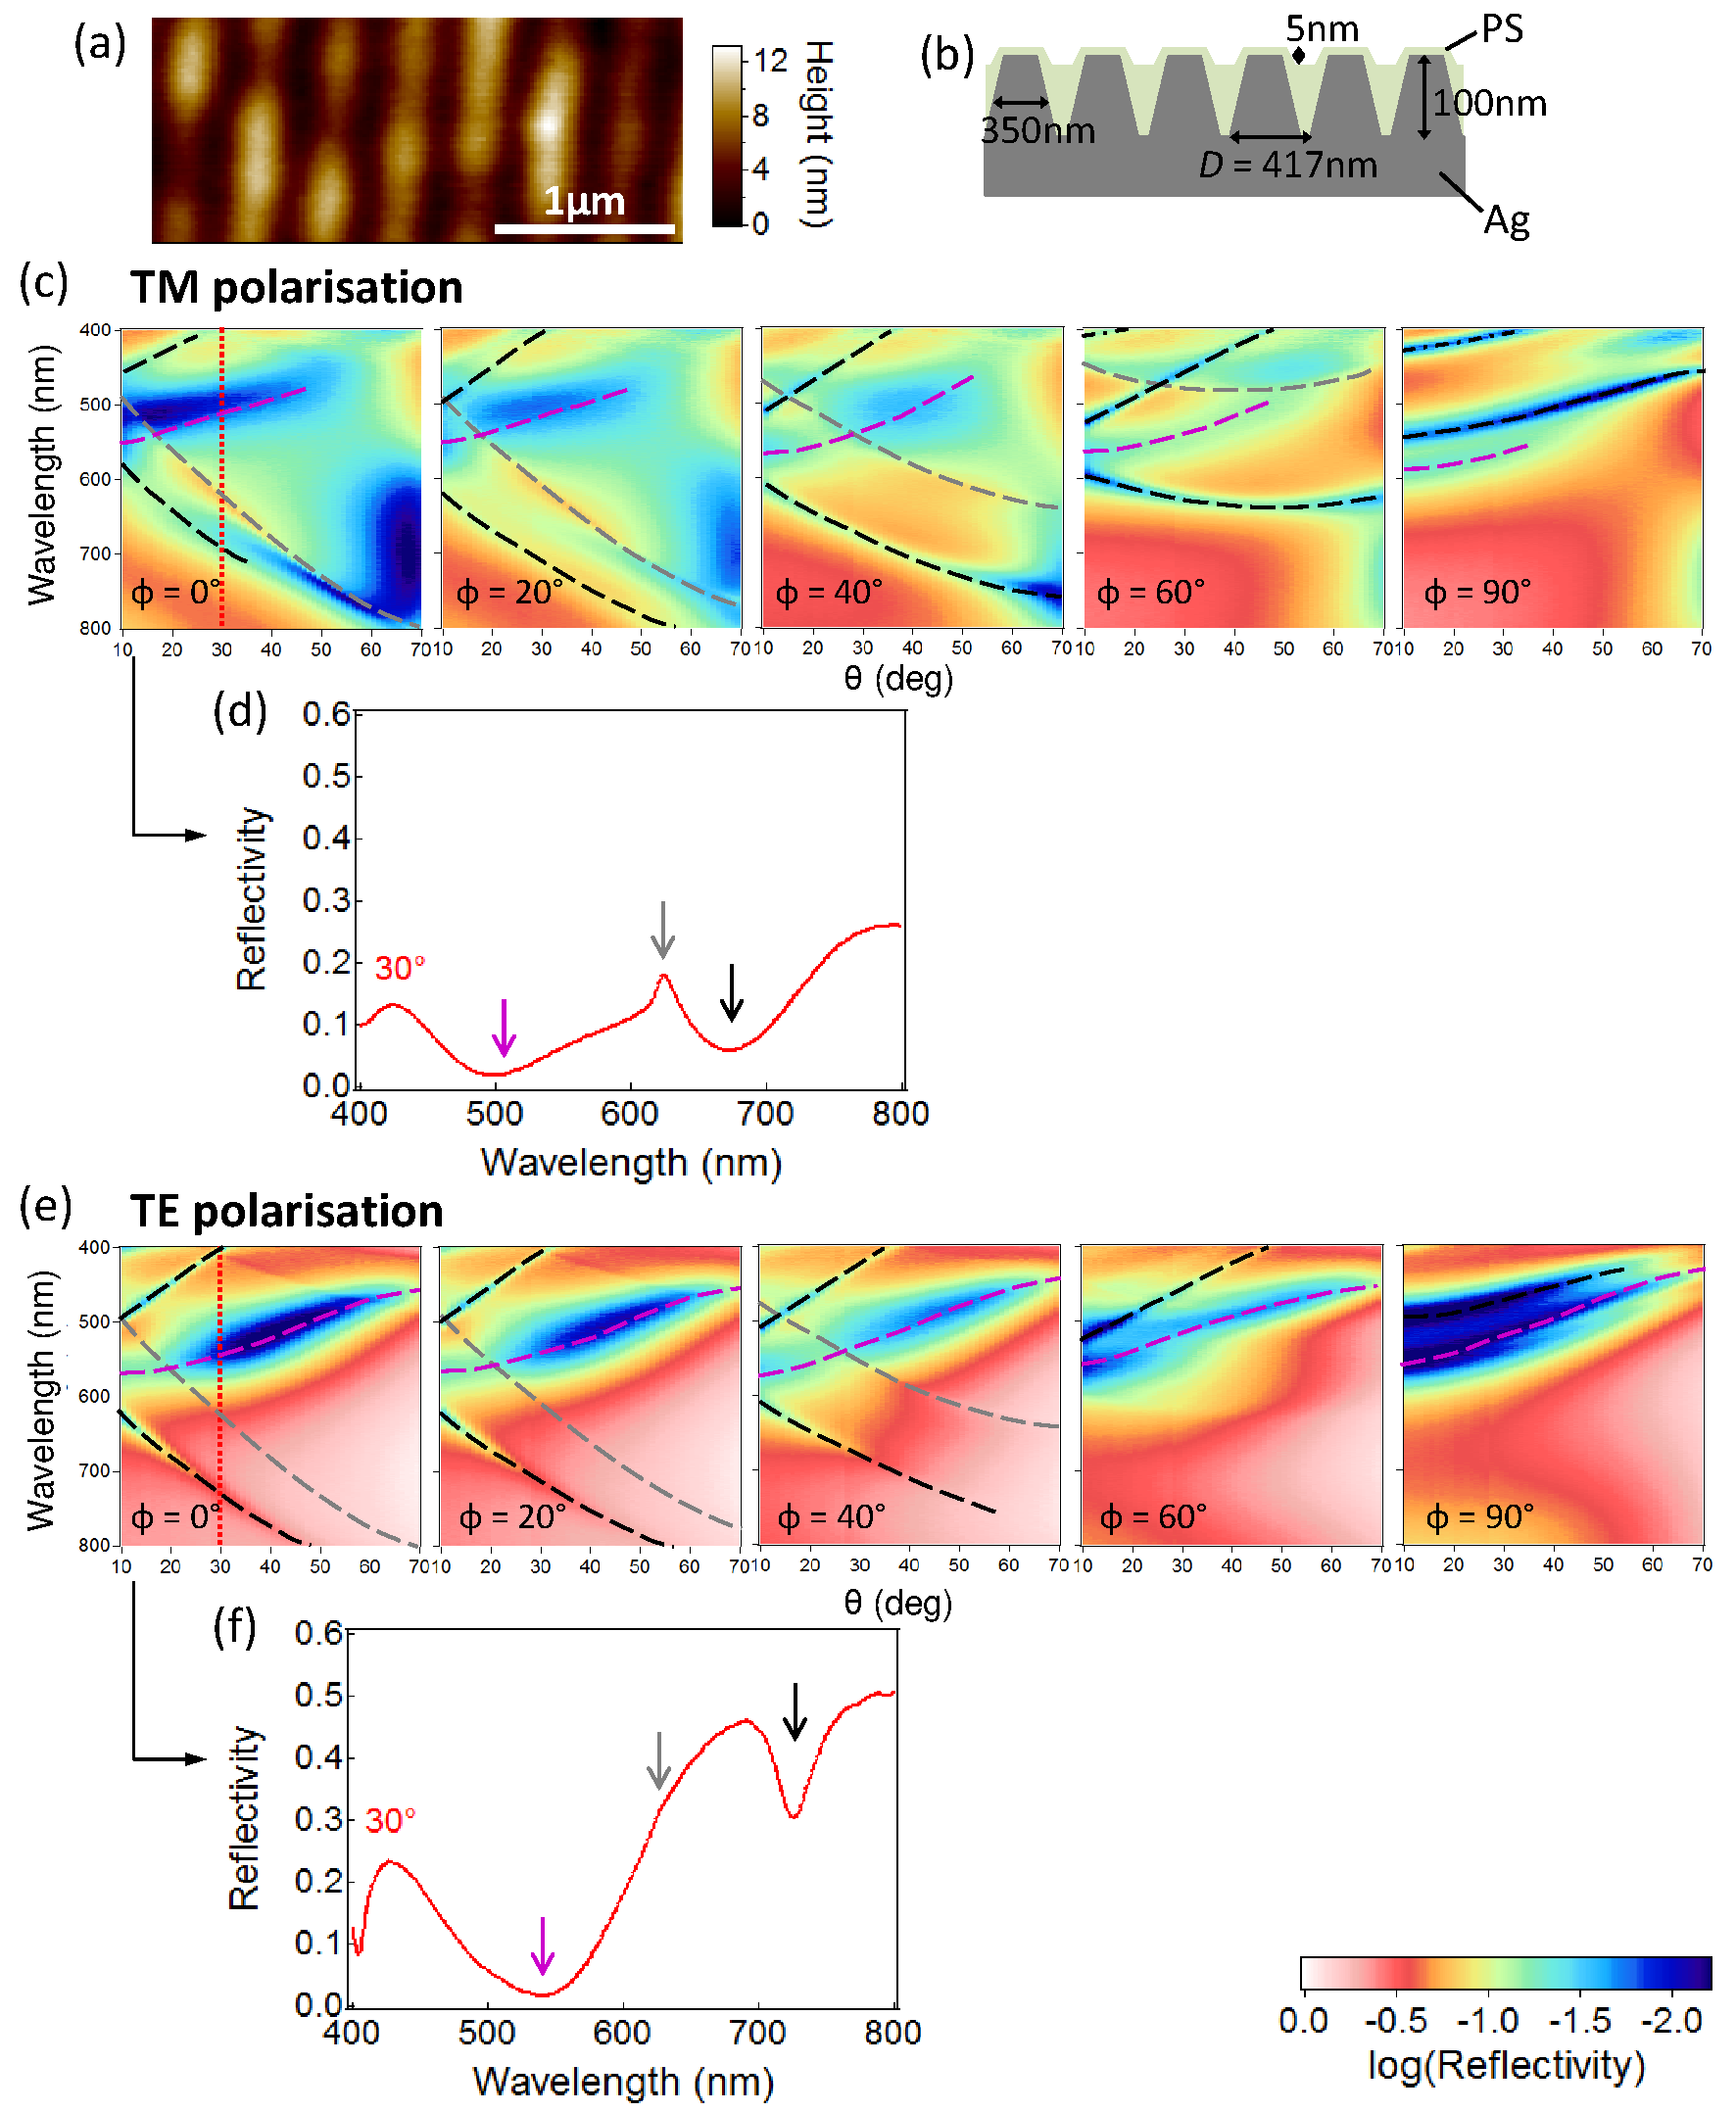
\includegraphics[width=0.95\textwidth]{Fig11}
\caption[(a) AFM image and (b) schematic structure of $D=417$\,nm PS-coated Ag grating. Reflectivity measurements of PS-coated Ag grating in (c,d) TM and (e.f) TE polarisation.]{(a) AFM image and (b) schematic structure of a $D=417$\,nm PS-coated Ag grating. (c) TM polarised reflectivity scans of the PS-coated Ag grating, and (d) reflectivity spectrum for $\phi=0^{\circ}$,\,$\theta=30^{\circ}$. (e,f) Same as above for TE polarisation. Photonic grating modes are indicated by grey lines/arrows on reflectivity scans/spectra, plasmonic gratings modes by black lines/arrows, and waveguide modes by purple lines/arrows.}
\label{7Fig11}
\end{figure}
\subsection{PS-coated Ag gratings}
From the AFM image of a $D=417$\,nm PS-coated grating [Fig.\,\ref{7Fig11}(a)] we see that the Ag grating is almost submerged beneath the non-uniform PS layer, resulting in a shallow sinusoidal surface grating with an average height of 5\,nm [Fig.\,\ref{7Fig11}(b)]. The presence of the PS overcoating increases the complexity of the reflectivity spectra by allowing access to more modes. In both TM and TE polarisations, photonic (grey dashed lines) and redshifted plasmonic modes (black dashed lines) can be observed [Fig.\,\ref{7Fig11}(c,e)], however the photonic mode is much weaker in TE polarisation. At high $\phi$ in TM polarisation, a second set of plasmonic modes can be seen (black dot-dashed lines), likely due to the differing PS thickness at the top and bottom surface of the grating. We also see a broader mode at $\sim560$\,nm for $\phi=0^{\circ}$,\,$\theta=10^{\circ}$ in both polarisations, which remains in roughly the same position for all $\phi$ (purple dashed line).

Using FEM, we observe two types of modes at $\phi=90^{\circ}$ in TM polarisation. A mode at higher energy has field intensity concentrated at the top surface of the grating, and evanescently decays from the Ag surface [Fig.\,\ref{7Fig12}(a)]. Taking snapshots throughout the optical cycle, the mode appears to be a quasiparticle travelling along the top surface of the grating [Fig.\,\ref{7Fig12}(b)]. By varying the geometry of the grating, we find the mode decreases in energy as $D$ increases, increases in energy with the slit width, and is unaffected by grating height. Thus this mode shows the behaviour expected for an SPP mode. On the other hand, the field intensity of the lower energy mode is mainly concentrated in the slit of the grating [Fig.\,\ref{7Fig12}(c)], and appears to travel along the slit [Fig.\,\ref{7Fig12}(d)]. The energy of the mode is unaffected by $D$ or the grating height, and decreases as the slit width increases. This behaviour is expected for a mode waveguided by the grating slit. According to Eq.\,\ref{waveguide} the dispersion fits that of a $\textnormal{TE}_{10}$ mode. 
\begin{figure}[h!p] 
\centering    
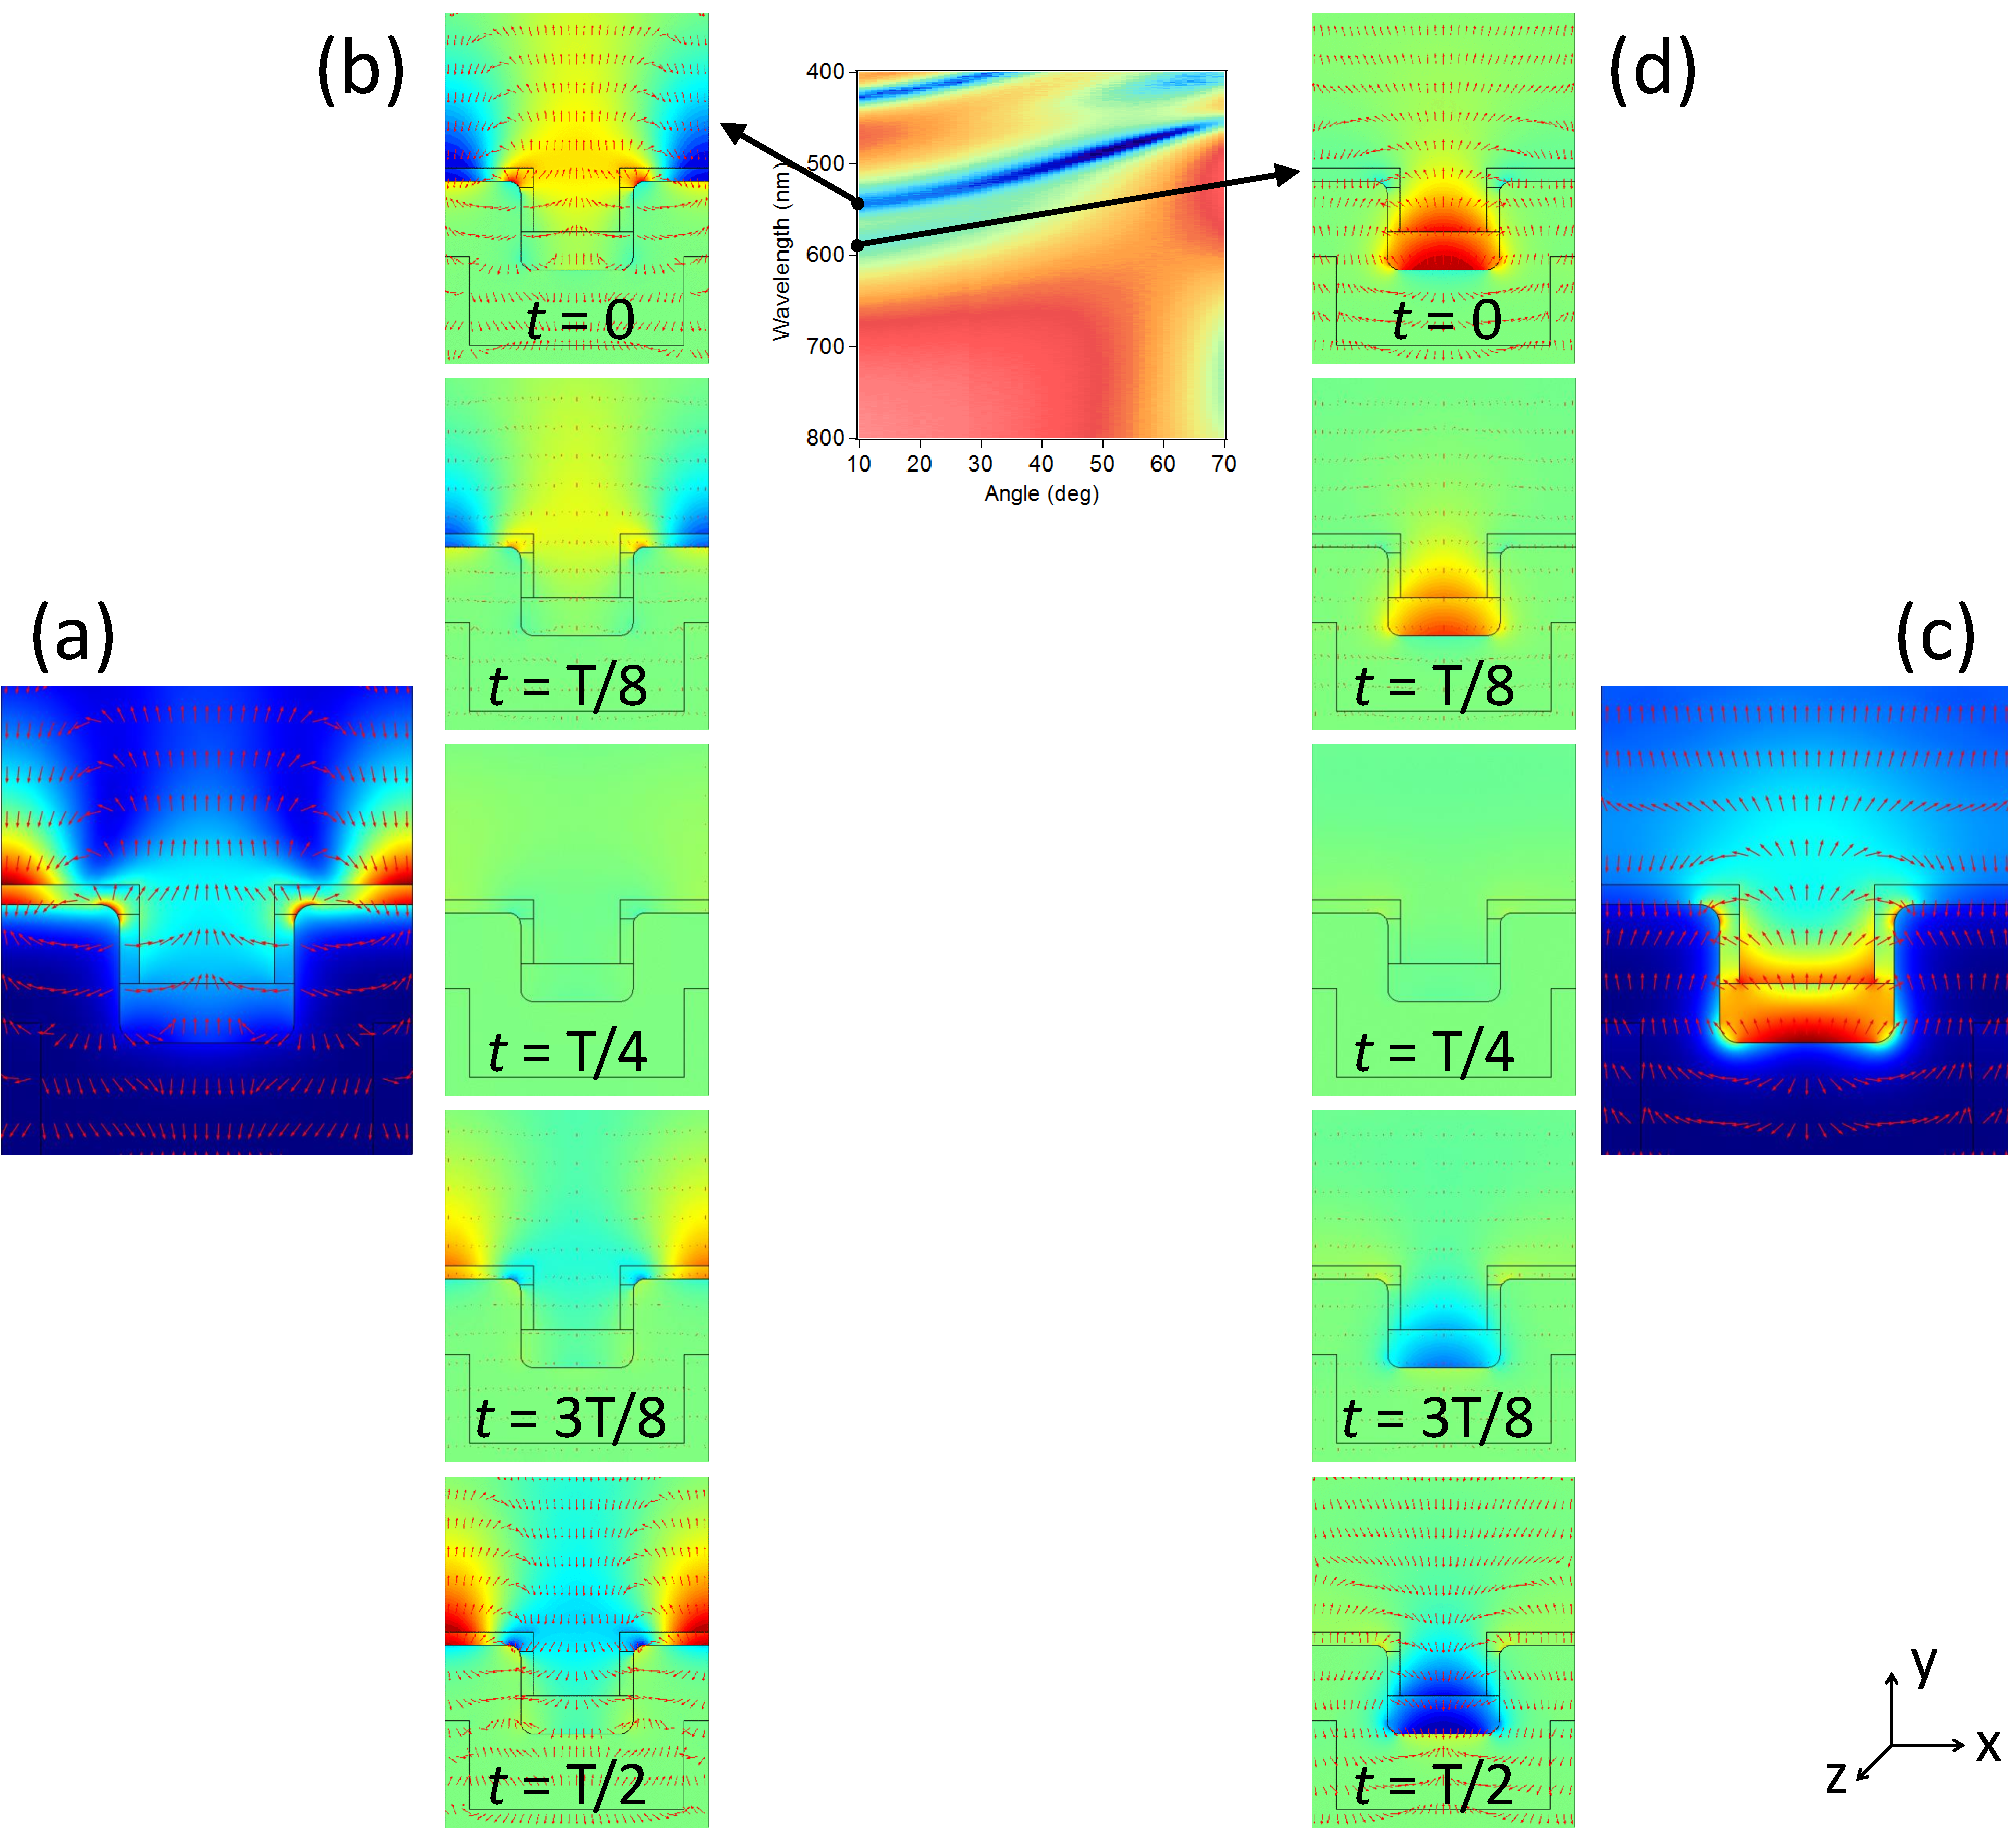
\includegraphics[width=\textwidth]{Fig12}
\caption{(a) Time averaged and (b) snapshots at time $t$ in the optical cycle T of the $E_y$ nearfield intensity for the higher energy (plasmonic) mode at $\phi=90^{\circ}$ $\theta=10^{\circ}$. (c,d) Same as above for the lower energy (waveguide) mode. Arrows represent the size and direction of the $\vec{E}$-field vector in the x-y plane. }
\label{7Fig12}
\end{figure}

Both SPP and waveguided modes are very sensitive to the dielectric environment as shown by Eqs.\,\ref{GratingDisp} and \ref{waveguide}, and Fig.\,\ref{7Fig13} shows the change in these modes with increasing PS thickness. Both the narrower SPP resonances (black dashed lines) and broader waveguided modes (purple dashed lines) redshift with increasing PS coverage as expected. For the structure in Fig.\,\ref{7Fig13}(c) these two modes actually overlap, although no interactions occur.
\begin{figure}[h!] 
\centering    
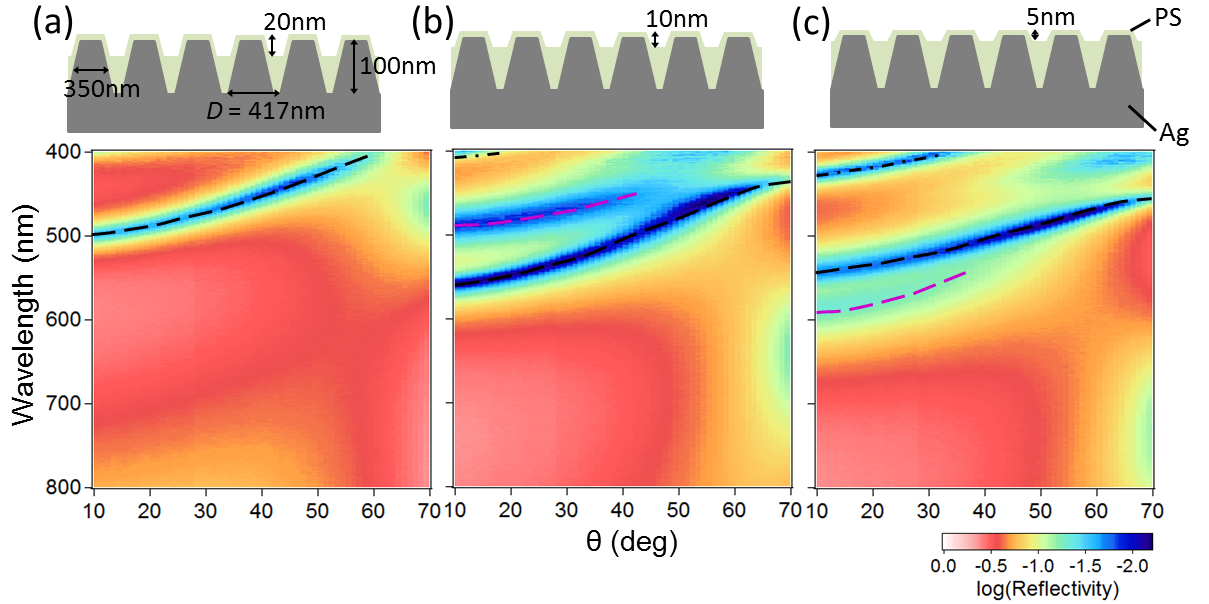
\includegraphics[width=\textwidth]{Fig13}
\caption{Schematic structure of PS-coated $D=417$\,nm Ag gratings (top), and TM polarised reflectivity scans at $\phi=90^{\circ}$ (bottom). PS thickness increases from (a) $\rightarrow$ (c). Plasmonic modes are indicated by black lines, and waveguide modes by purple lines.}
\label{7Fig13}
\end{figure}

\begin{figure}[h!] 
\centering    
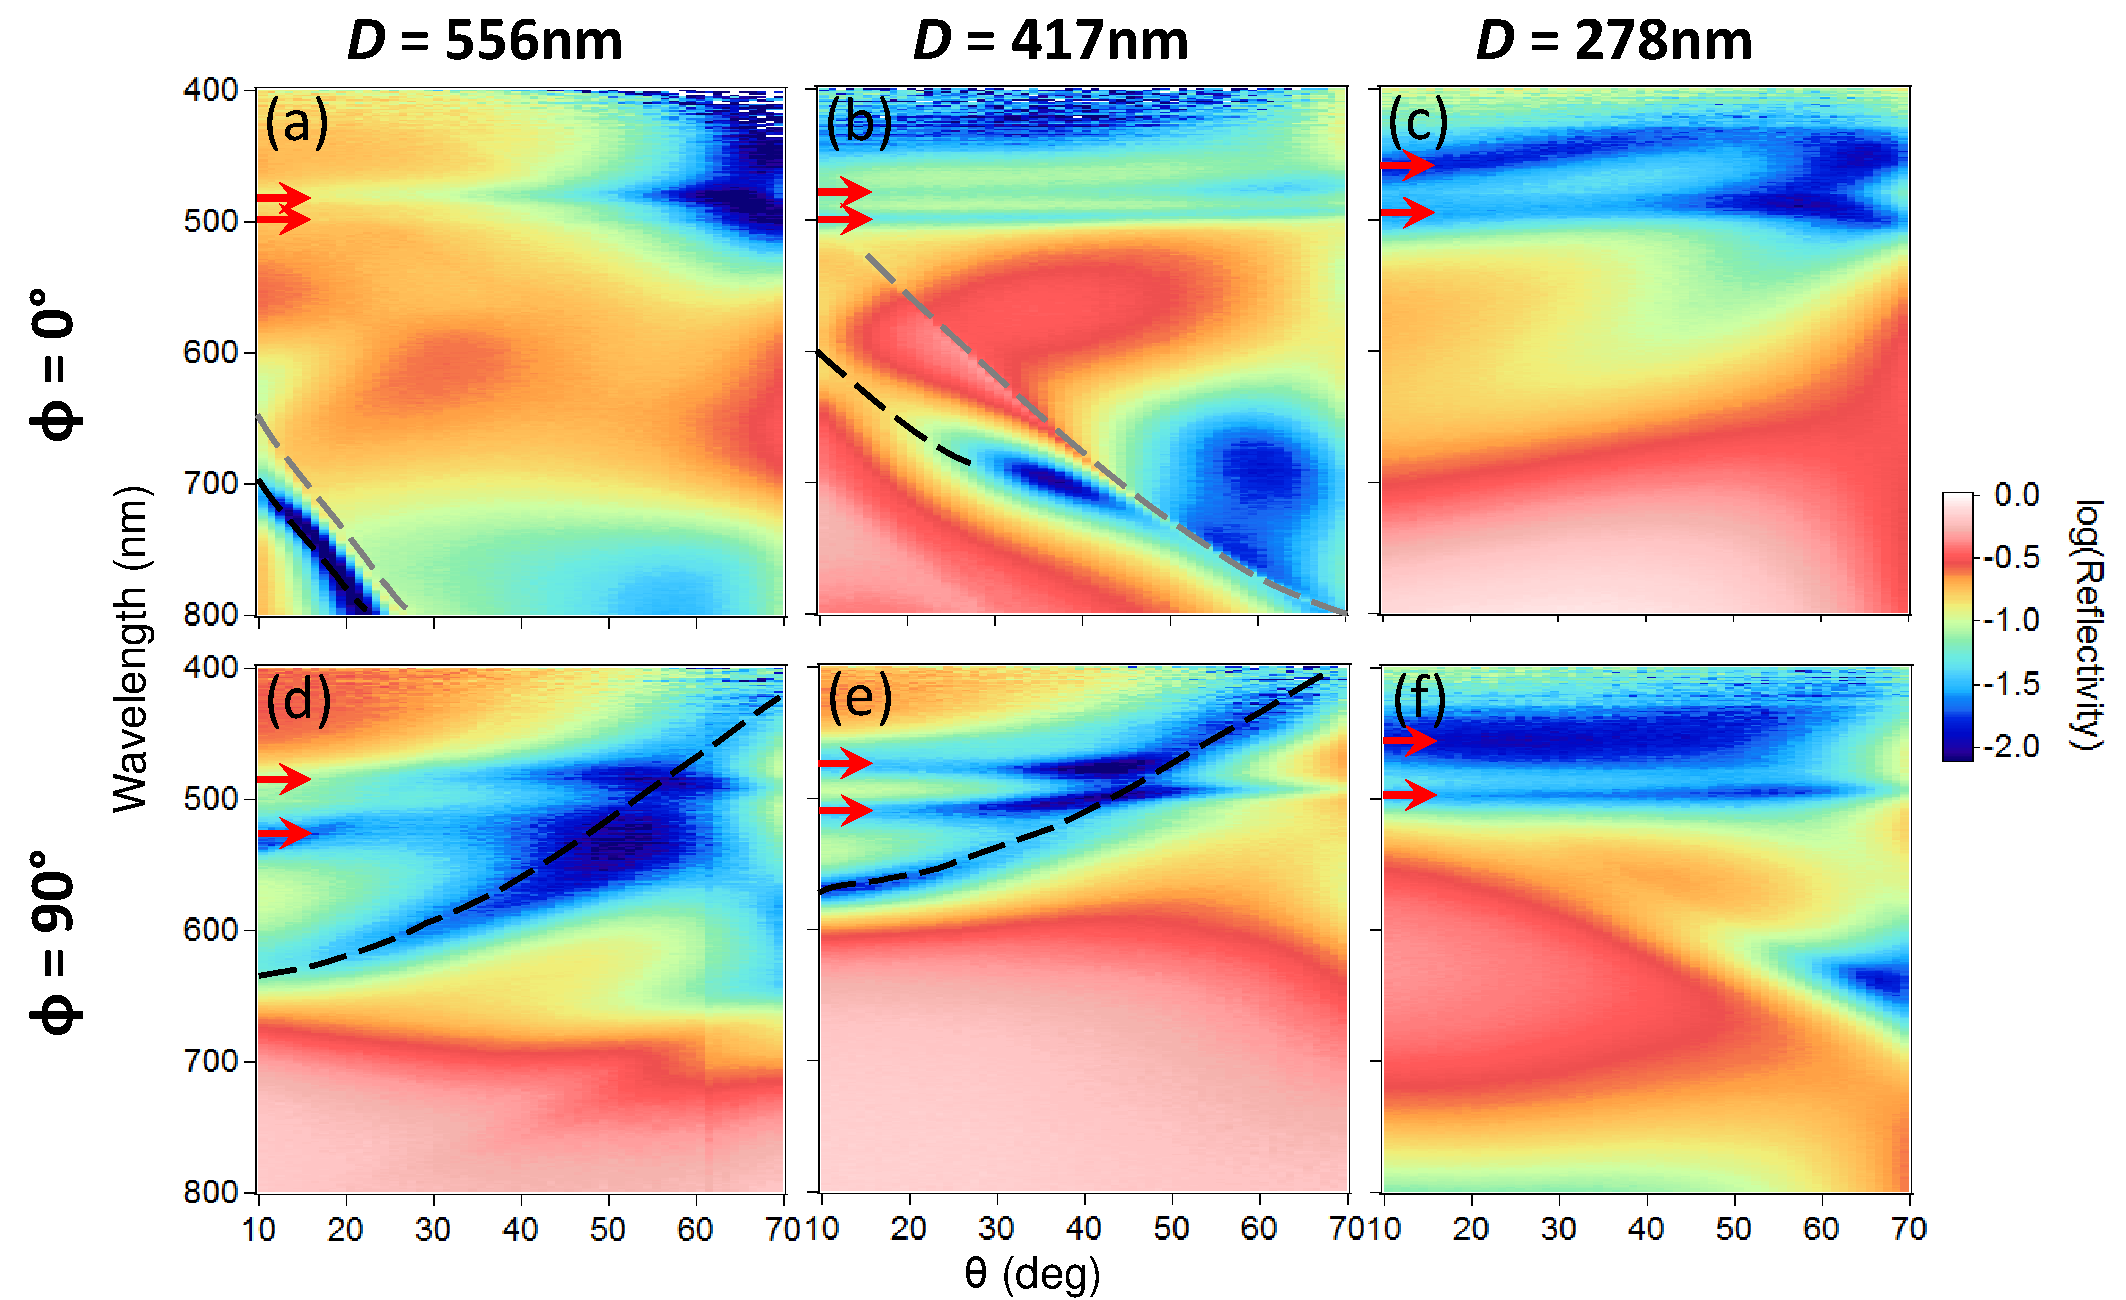
\includegraphics[width=\textwidth]{Fig14}
\caption{TM specular reflectivity scans of CHPI-coated Ag gratings with $D$ and $\phi$ as labelled. Photonic grating modes are marked by grey dashed lines, plasmonic grating modes by black dashed lines, and excitons indicated by red arrows.}
\label{7Fig14}
\end{figure}

\subsection{CHPI-coated Ag gratings}
Fig.\,\ref{7Fig14} shows TM reflectivity scans for CHPI-coated Ag gratings, $D=556$, 417 and 278\,nm at $\phi=0$ and $90^{\circ}$. The spectra for $D=556$ and 417\,nm are very similar, showing two exciton modes (red arrows) that strongly couple to an SPP grating mode (black dashed line) as the oscillations become resonant at $\phi=90^{\circ}$. Two excitons can also be observed for $D=278$\,nm, however the SPP mode is at a higher energy and thus the coupling occurs at $\phi=0^{\circ}$.

TM polarised reflectivity scans of a $D=417$\,nm CHPI-coated Ag grating at $\phi=0^{\circ}$ [Fig.\,\ref{7Fig15}(a)] show two dispersionless exciton modes at 480 and 500\,nm (marked by arrows) far off resonance with grating modes. The persistent presence of a second exciton is only detected when SPPs can be excited, i.\,e.\,in TM polarisation [Fig.\,\ref{7Fig15}(a)] but not TE [Fig.\,\ref{7Fig15}(b)], nor in CHPI-coated planar Ag films [Fig.\,\ref{7Fig15}(c)]. It is also not observed for CHPI-coated non-plasmonic gratings [Figs.\,\ref{7Fig3} and \ref{7Fig6}], thus from Fig.\,\ref{7Fig15} we deduce that SPP excitation leads to the observation of an additional redshifted exciton with a splitting of 100\,meV. Its appearance only when SPPs are present rules out any influence from modified CHPI assembly in the grooves, which are in any case hundreds of times larger than the PbI layer spacing. In addition the exciton diffusion length in 2D perovskites is of order 10\,nm \cite{Ahmad2013}, therefore we do not expect any limiting effects due to the grating geometry. We note slight changes in the CHPI coverage alter the positions and intensities of dispersive grating modes [\textit{cf} Fig.\,\ref{7Fig17}(c), with a thinner CHPI coating], however the exciton modes remain essentially unchanged.

\begin{figure}[h!] 
\centering    
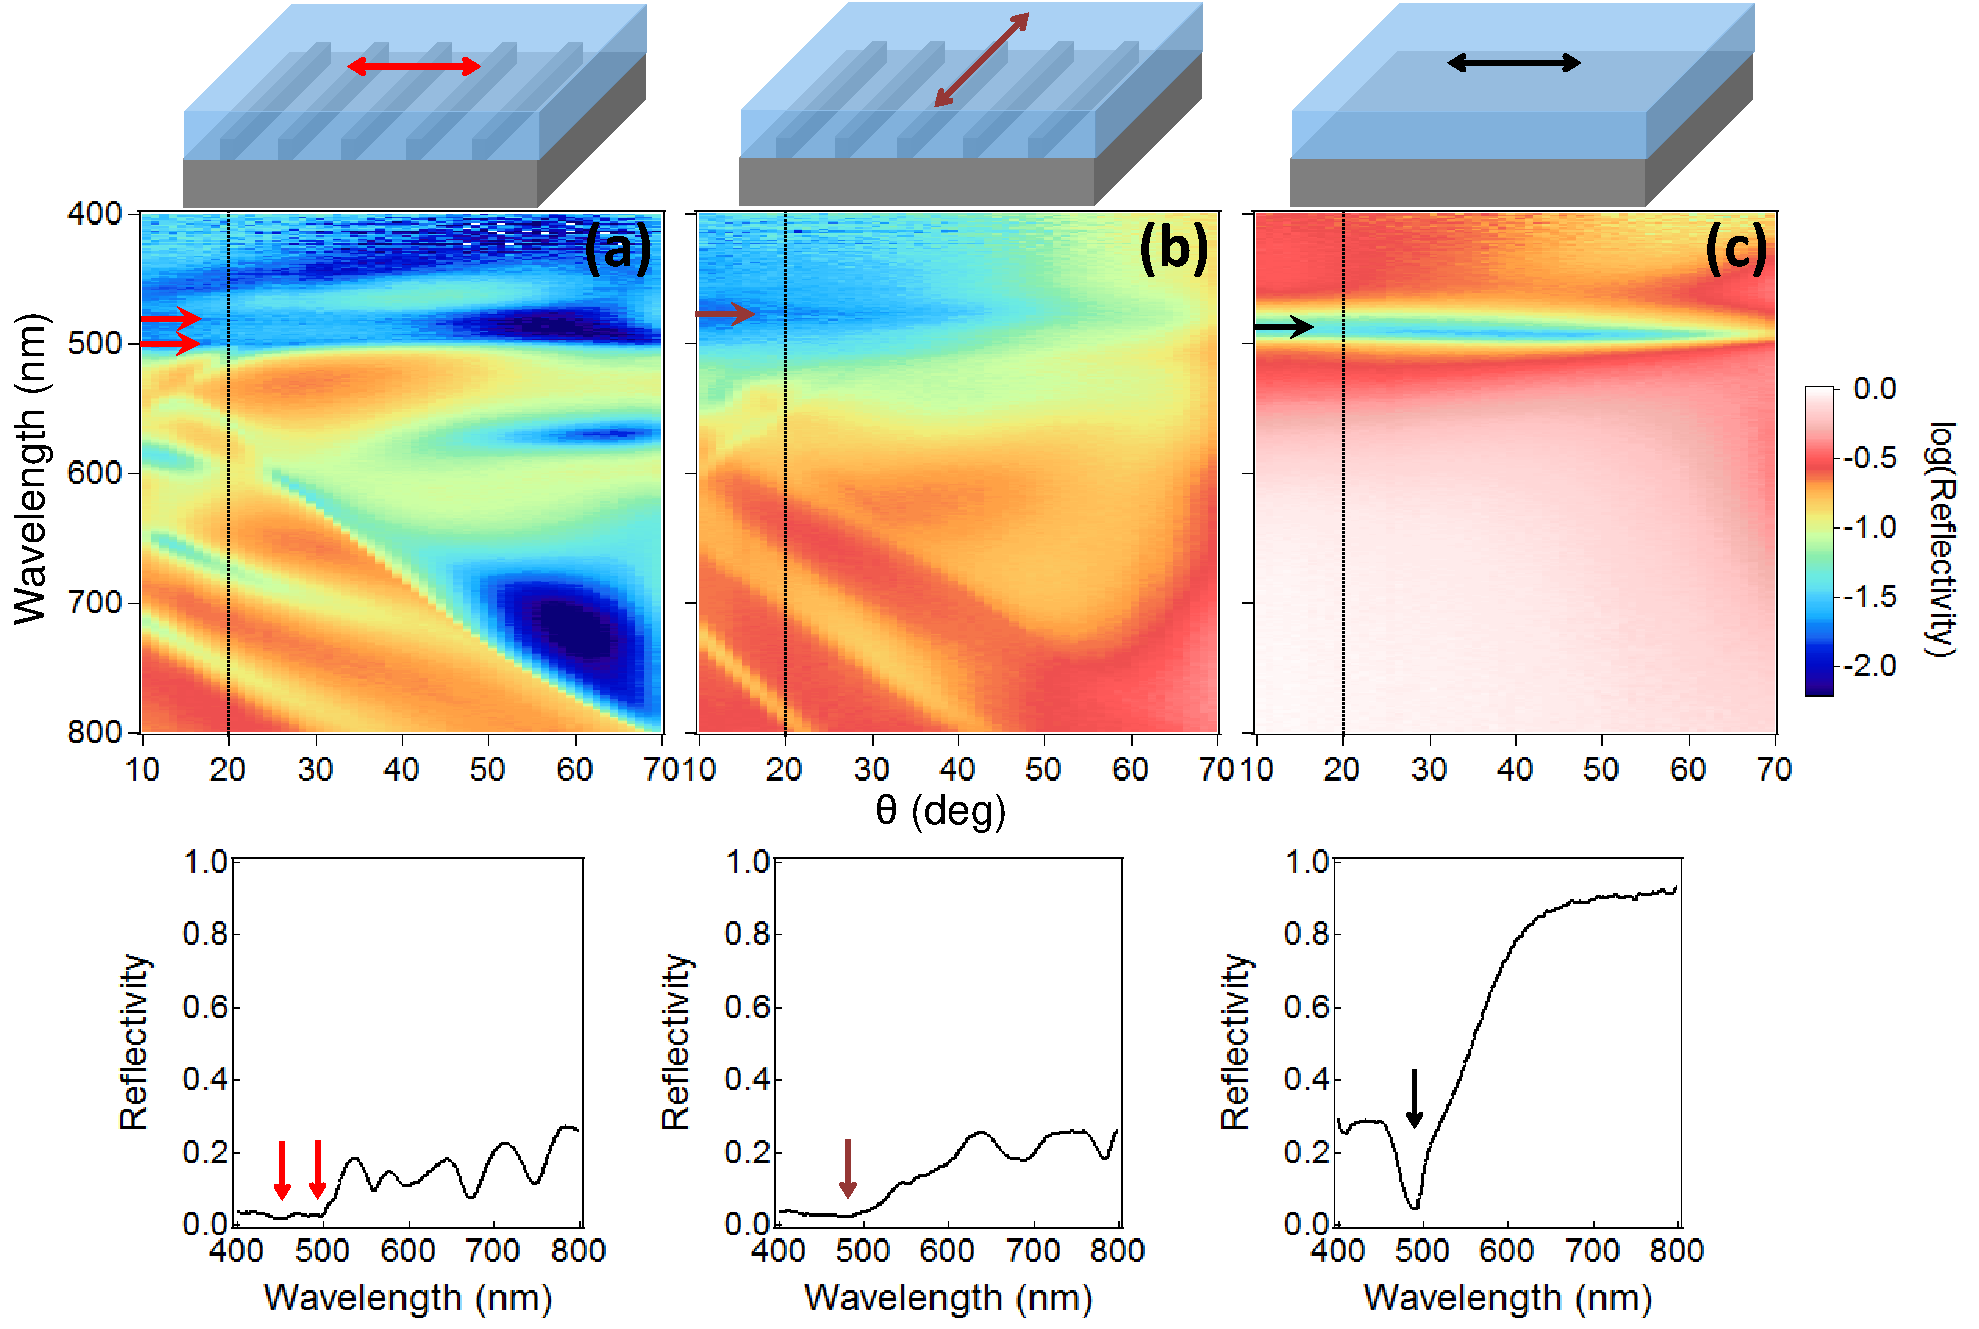
\includegraphics[width=\textwidth]{Fig15}
\caption{Specular reflectivity scans at $\phi=0^{\circ}$: CHPI-coated Ag grating with (a) TM and (b) TE polarised light, and (c) CHPI-coated 120\,nm planar Ag film with TM polarised light. The $\vec{E}$-field orientation is shown above each scan, the reflectivity spectra at $\theta=20^{\circ}$ below, and positions of exciton modes are indicated by arrows.}
\label{7Fig15}
\end{figure}

It is well known that the emitted energy of a dipole (exciton) is lowered when placed in front of a metallic surface due to interactions between the dipole and the reflected electromagnetic field \cite{Morawitz1969, Morawitz1974, Chance1974, Chance1975, Chance1975a, Ford1984}. Using the method of images, we can replace the metal and describe instead the coupling between an exciton in the CHPI ($\epsilon_1$) and its image exciton in the metal ($\epsilon_2$), modified by their respective dielectric environments. Chance \textit{et al.} \cite{Chance1975} showed the redshift in the emitted energy of an exciton ($\Delta E_{ex}$) oriented parallel to the interface can be approximated by
\begin{equation}
\centering
\Delta E_{ex} \sim \left( \frac{1}{k_1 l} \right) ^3 \text{Re} \left\{ \frac{\epsilon_2 - \epsilon_1}{\epsilon_2 + \epsilon_1} \right\} q \Gamma_0 ,
\label{Redshift}
\end{equation}
where $l$ is the distance between the exciton and a metal surface, $k_1$ is the wavenumber of light in CHPI, $q$ is the quantum yield of CHPI excitons (taken here to be 1), and $\Gamma_0$ is the inverse exciton radiative lifetime without the metal. Similar to the appearance of excitons in the spectra, we expect to observe such coupled `image-biexcitons' as minima in the reflectivity, at a wavelength that differs from the uncoupled exciton according to Eq.\,\ref{Redshift}. The strength of coupling between the exciton and reflected electromagnetic field depends on the exciton dipole moment, which is controlled by the term $q \Gamma_0$. From this we can see the $l^{-3}$ dependence of the redshift as shown in Fig.\,\ref{7Fig16}(a), where the experimentally observed $\Delta E_{ex} \negmedspace \sim \negmedspace 100$\,meV corresponds to $l \negmedspace \sim \negmedspace 22$\,nm, close to the experimentally-determined CHPI thickness. Clearly $\Delta E_{ex}$ is also affected by the dielectric response of CHPI and Ag, and from Eq.\,\ref{Redshift} we see that $\Delta E_{ex}$ is maximised if $\epsilon_2 + \epsilon_1 \rightarrow 0$, i.\,e.\,when emission is resonant with an SPP on the metal-dielectric interface. The linewidth of %WN
the exciton is also affected by interactions with image charges in the metal, however in our perovskite system this effect is not dominant due to tight planar confinement of excitons. We expect larger effects in systems that are less perfectly 2D, such as semiconductor heterostructures and J-aggregate systems, where surface charges play a much larger role.

\begin{figure}[h!] 
\centering
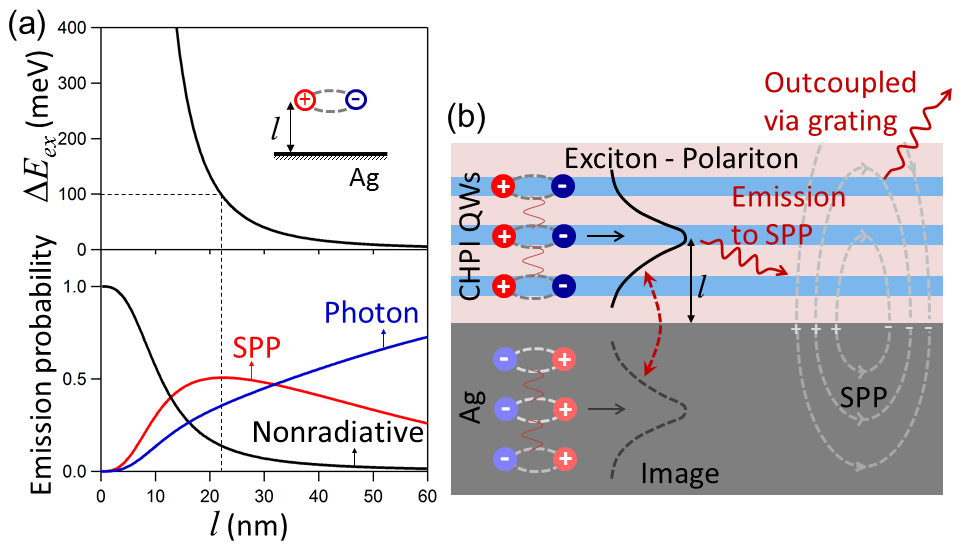
\includegraphics[width=0.9\textwidth]{Fig16}
\caption{(a) Change in emitted energy (top) and relative decay probabilities (bottom) of an exciton with energy 2.6\,eV placed distance $l$ from the Ag surface. The dashed line indicates the experimentally measured redshift. (b) Schematic mechanism for SPP-mediated emission of image-biexciton.}
\label{7Fig16}
\end{figure}
The role of the SPP in this case is to outcouple the signal of the redshifted exciton. There are three main decay channels for dipole emission near a metal surface: direct emission to photons, emission to SPPs, and nonradiative processes such as the excitation of electron-hole pairs and lossy surface waves on the metal. Other nonradiative paths via defects or phonons are independent of $l$ and will be ignored in this analysis. Emission into SPPs provides an extra radiative decay channel as this signal can be extracted to the far field via the periodic nanostructure, and this mechanism has been used to improve the luminescence efficiency of light emitting devices \cite{Frischeisen2011, Kumar2012}. The relative decay probability for each process is calculated as a function of $l$ \cite{Ford1984} and shown in Fig.\,\ref{7Fig16}(a). Although these calculations are intended for SPPs propagating on planar metal surfaces, we can use them as approximations for our grating system, although we note such estimates are indeed expected to become less accurate with increasing structure depth. Up to a CHPI thickness of 25\,nm, SPP mediated emission is the most important radiative decay channel with a maximum emission probability at 22\,nm, matching the experimentally observed $\Delta E_{ex}$. Even for thicker CHPI films we expect the exciton modes to remain at the same positions, because SPP emission becomes weak at large $l$ where $\Delta E_{ex}$ is negligible.

In our MQW perovskite system, localised excitons in periodically-spaced nearby QWs are optically coupled together to form collective exciton-polariton states an average distance $l$ from the Ag surface \cite{Pbbr2008, Baumberg1998, Kavokin1998, Vladimirova1998}. Therefore in CHPI-coated Ag gratings we observe both in-plane exciton-polaritons, and out-of-plane interactions that lead to `image-biexcitons', which are outcoupled via SPP emission with a binding energy of 100\,meV at room temperature [Fig.\,\ref{7Fig16}(b)]. For our grating system, the exciton and SPP modes become closer in energy with increasing $\phi$ [see below and Fig.\,\ref{7Fig17}(c)], and as a result splitting between the exciton modes (indicated by arrows in Fig.\,\ref{7Fig17}(c)) increases to around 185\,meV at $\phi=90^{\circ}$. The azimuthal dependence of the exciton splitting reflects the tuneable modification of the Coulomb interaction in this geometry, but however requires further theoretical development.

\begin{figure}[h!] 
\centering    
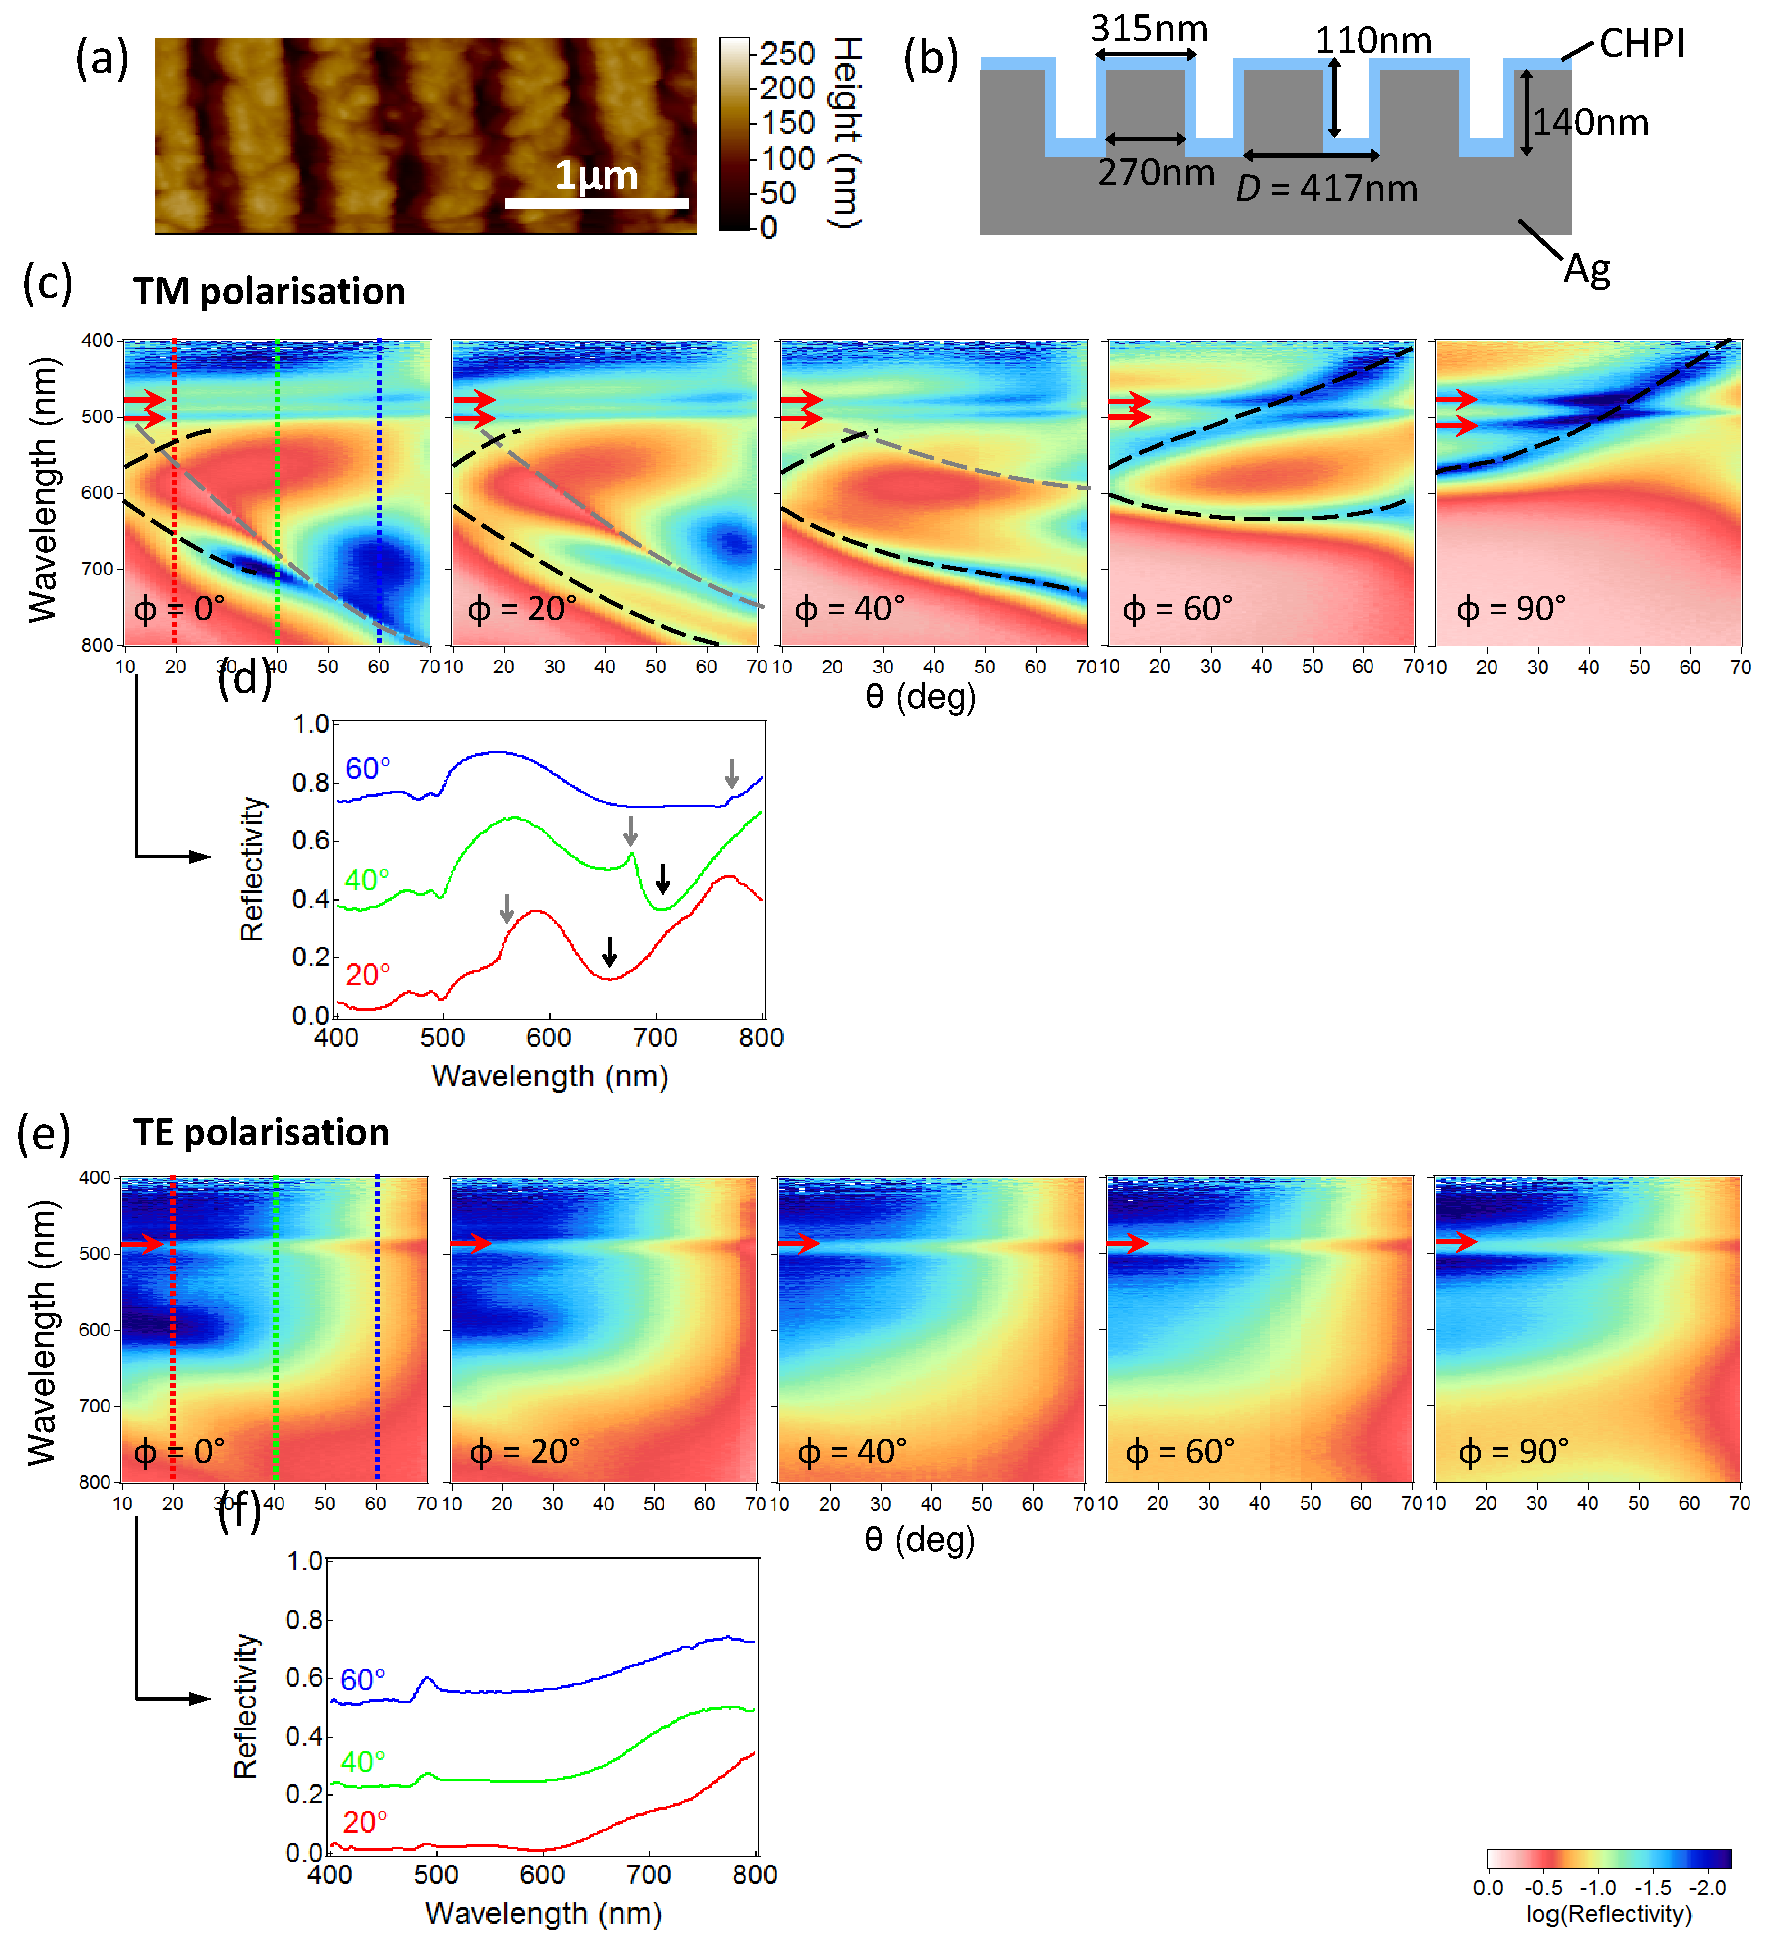
\includegraphics[width=0.95\textwidth]{Fig17}
\caption[(a) AFM image and (b) schematic structure of $D=417$\,nm CHPI-coated Ag grating. Reflectivity measurements of CHPI-coated Ag grating in (c,d) TM and (e.f) TE polarisation.]{(a) AFM image and (b) schematic structure of a $D=417$\,nm CHPI-coated Ag grating. (c) TM polarised reflectivity scans of the CHPI-coated Ag grating, and (d) reflectivity spectra for $\phi=0^{\circ}$. Spectra are offset for clarity. (e,f) Same as above for TE polarisation. Photonic grating modes are indicated by grey lines/arrows on reflectivity scans/spectra, plasmonic gratings modes by black lines/arrows, and excitons by red arrows.}
\label{7Fig17}
\end{figure}

AFM image of a $D=417$\,nm CHPI-coated Ag grating shows a clear grating structure despite the roughness of CHPI coating [Fig.\,\ref{7Fig17}(a)]. Using AFM measurements, we find CHPI forms a conformal coating around the Ag grating with thickness $\sim25$\,nm [Fig.\,\ref{7Fig17}(b)]. In TE polarisation, we only observe the presence of one exciton without the signature of any grating modes, similar to the CHPI-coated Ti gratings. In TM polarised reflectivity scans, as well as strong %WN
excitons %end
(red arrows) we also observe $m=\pm1$ photonic and plasmonic grating modes [Fig.\,\ref{7Fig17}(c)].  As the SPP modes become resonant with the exciton and image exciton, the light-matter modes strongly couple and produce an anticrossing in the reflectivity of 0.25\,eV. Extracting the mode positions from the $\phi=90^{\circ}$ scan [Fig.\,\ref{7Fig17}(c)] allows them to be fit to a three oscillator model using the Hamiltonian
\begin{equation}
\centering 
\hat{H}=\left( \begin{matrix} 
E_{ex} & 0 & \Omega_{ex}/2 \\
0 & E_{bx} & \Omega_{bx}/2 \\
\Omega_{ex}/2 & \Omega_{bx}/2 & E_{pl} 
\end{matrix} \right) ,
\end{equation}
where $E_{ex}$, $E_{bx}$ and $E_{pl}$ are the energies of the exciton-polariton, image-biexciton and plasmonic grating modes respectively, while $\Omega_{ex}$ and $\Omega_{bx}$ represent the interaction between the SPP and exciton/image-biexciton. From this we find Rabi splittings of $\Omega_{ex}=150$\,meV and $\Omega_{bx}=125$\,meV. 
These are greatly enhanced because of the large confinement of the plasmonic optical field in the thin PbI QW layers. The Rabi splitting is given by $\Omega \propto \sqrt{f_{osc} N_{QW}/V}$, where the oscillator strength ($f_{osc}$) of the CHPI is assumed to be similar for coupling to photons or plasmons, the number of QWs ($N_{QW}$) is proportional to the CHPI thickness, and the mode volume ($V$) is here proportional to the optical mode size. Comparing to Fabry-Perot planar CHPI microcavities in strong coupling \cite{Pradeesh2009b} which have CHPI thickness of 72\,nm, cavity length of 407\,nm, and a Rabi frequency of $\Omega_{FP}=65$\,meV, the simple scaling above predicts $\Omega_{SPP} \sim \Omega_{FP} \sqrt{(22/72).(407/22)}$=156\,meV, in excellent agreement with our measurements. Using SPPs to strongly couple to the excitons thus dramatically reduces the cavity length, thus enhancing the light-matter coupling.


\begin{figure}[h!] 
\centering    
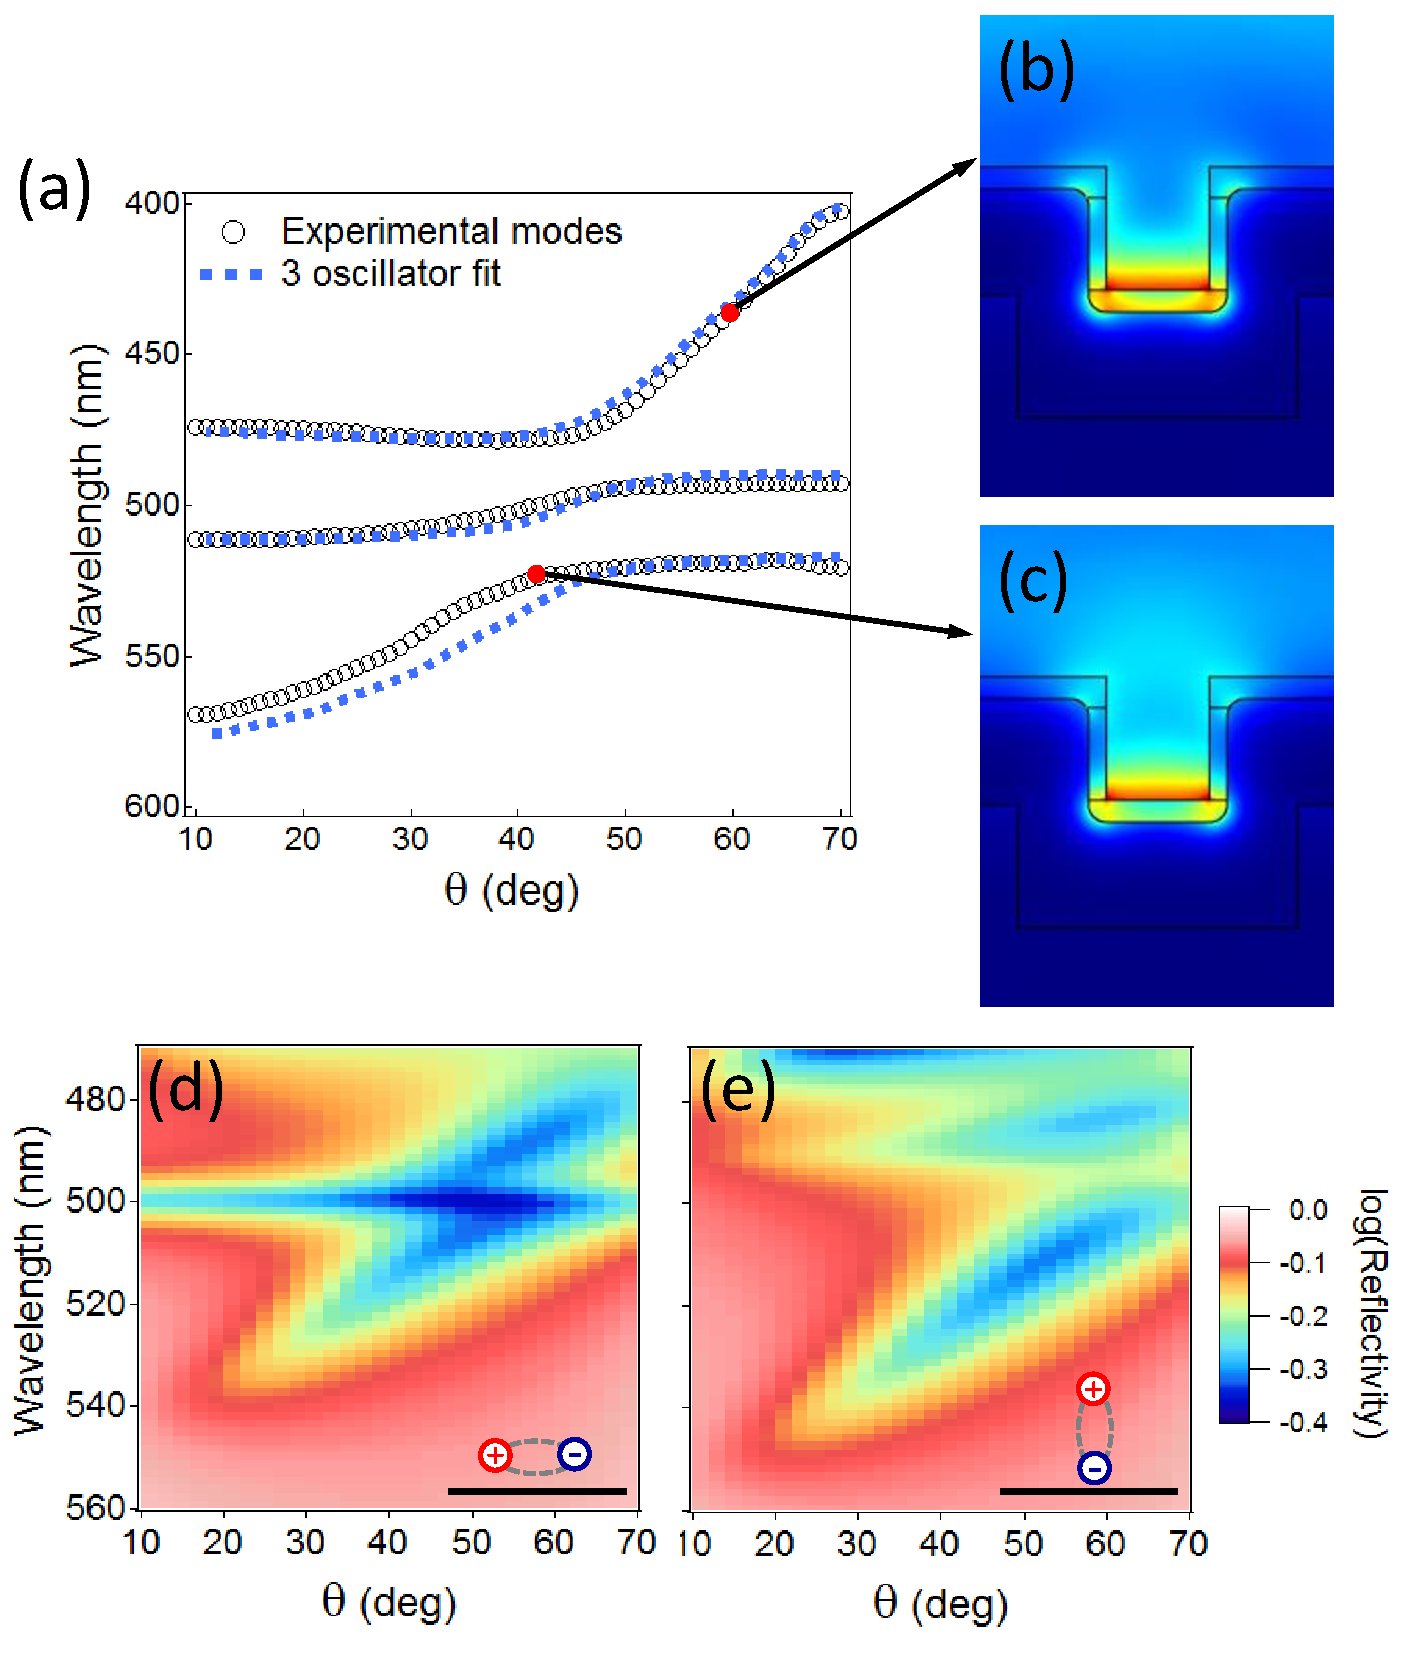
\includegraphics[width=0.8\textwidth]{Fig18}
\caption{(a) Extracted spectral mode positions for $\phi=90^{\circ}$ reflection dips (open circles), and fit from three oscillator coupling model (dashed lines). (b,c) Time-averaged $\vec{E}$-field intensity profiles ($\vec{E}\cdot\vec{E}$) as indicated. (d,e) Simulated reflection spectra for (d) in-plane and (e) out-of-plane exciton dipoles.}
\label{7Fig18}
\end{figure}
We calculate the full eigenstates of the system using FEM simulations. These confirm the anticrossings observed, and provide the optical field profiles.
In the case of strong coupling at $\phi=90^{\circ}$, the time-averaged near-field shows strongest intensity inside the CHPI which coats the bottom surface of the grating, with a rapid evanescent decay away from the interface [Figs.\,\ref{7Fig18}(b,c)]. The mode is thus both laterally confined by the grating as well as being trapped inside the surface layers where it couples to the excitons.

The SPP $\vec{E}$-field direction is primarily perpendicular to the metal-dielectric interface, while excitons in CHPI QWs are polarised parallel to this interface \cite{Pradeesh2009b, Mitzi2001b}.  Simulated $\phi=90^{\circ}$ spectra for in- and out-of-plane exciton dipoles are shown in Figs.\,\ref{7Fig18}(d,e) respectively. While strong coupling is seen for both dipole orientations, the bare exciton is only seen for the in-plane dipole. It thus appears that the coupling between the excitons and their images are responsible for mixing the dipole orientations, enabling the strong coupling with the SPP mode. Far-field light is directly coupled into the layered perovskite system, where the excitons mediate SPP interactions. The polariton states mix excitons within the perovskite which are delocalised across many PbI monolayers, with SPPs which are tightly confined to the CHPI layer above the Ag grating and laterally localised in the grating slits by the coupling of standing waves. Such light-matter polaritonic quasiparticles thus combine organic, inorganic and plasmonic components in an unusual fashion.


\section{Conclusions}
Simple plasmonic periodic structures give rise to a wide range of grating modes: photonic modes due to the interference of light, excitement of SPPs on the surface of the metal, and laterally localised modes such as channel plasmons or waveguided modes. The positions and efficiencies of many of these modes are sensitive to the geometry of the grating and the dielectric environment provided by any overcoating materials.

In CHPI-coated Ag gratings, we observe evidence of image-biexcitons with binding energy 100\,meV at room temperature. Such quasiparticles arise from the interaction between excitons and their images in the metal, and are outcoupled from the grating structure via SPP emission. These out-of-plane biexciton states mediate coupling between in-plane QW excitons and out-of-plane SPP grating modes. This enables the observation of strong coupling at room temperature with Rabi splittings of 150 and 125\,meV for the exciton and image-biexciton respectively. Both the biexciton binding energy and strong coupling Rabi splitting is tunable by small changes in the structure of the coated gratings.

Strong coupling has previously been observed between inorganic or organic excitons and Au nanoslit gratings at low temperature. The coupling constants in these systems are much smaller compared to CHPI at room temperature: 55\,meV for 50\,nm J-aggregate films at 77\,K \cite{Vasa2010}, and 8\,meV for 10\,nm GaAs QWs at 10\,K \cite{Vasa2008}. One key difference is that for the III-V semiconductors the QWs have to be spaced at least 20\,nm from the metal surface to maintain their optical quality. In contrast our 25\,nm thick CHPI film is prepared directly on the metal, and still gives strongly radiative exciton modes because the organic sandwich protects the PbI QW layers. Theoretically Fig.\,\ref{7Fig16}(a) shows that excitons remain radiative via SPP coupling for film thickness above 10\,nm. Hence the perovskite system is well suited to manipulate light-matter interactions. Such modification of exciton behaviour is of great interest for other layered van der Waals semiconductors such as derivatives of graphene and transition metal dichalcogenides, particularly for future optoelectronic devices that demand large field enhancements by coupling to SPPs.